\documentclass[12pt,a4paper]{report}
\usepackage[margin=25mm]{geometry}
\usepackage{graphicx}
\usepackage{float}
\usepackage{amsmath,amssymb}
\usepackage{booktabs}
\usepackage{array}
\usepackage{hyperref}
\usepackage{xcolor}
\usepackage{enumitem}
\usepackage{caption}
\usepackage{listings}

\graphicspath{{report_figures/}}
\hypersetup{colorlinks=true, linkcolor=blue, citecolor=blue, urlcolor=blue}
\setlist{nosep}

\lstset{
  basicstyle=\small\ttfamily,
  breaklines=true,
  frame=single,
  columns=fullflexible
}

\newcommand{\figwidth}{0.86}
\newcommand{\sincos}{\operatorname{sincos}}

\begin{document}

\begin{titlepage}
  \centering
  \vspace*{1.8cm}
  {\Large University of Cambridge Department of Engineering\par}
  \vspace{1.5cm}
  {\Huge\bfseries Neuromorphic Bat-Inspired 3D Echolocation for Edge Localisation\par}
  \vspace{1.2cm}
  {\Large Full Draft Report\par}
  \vfill
  \begin{tabular}{ll}
    Name: & \textit{[Your name]}\\
    College: & \textit{[Your college]}\\
    Supervisor: & \textit{[Supervisor]}\\
    Project title: & Neuromorphic Bat-Inspired 3D Echolocation for Edge Localisation\\
    Date: & \today
  \end{tabular}
\end{titlepage}

\pagenumbering{roman}
\chapter*{Technical Abstract}
\addcontentsline{toc}{chapter}{Technical Abstract}

This project investigates a biologically inspired approach to three-dimensional echolocation for low-power edge systems. The engineering task is to estimate target distance, azimuth, and elevation from an emitted frequency-modulated acoustic call and its returned echo. Conventional sonar pipelines can solve this problem through high-resolution sampling, explicit cross-correlation, beamforming, and trained regression. However, these methods are not naturally sparse and can become expensive when the computation must run continuously on an embedded platform. Bat echolocation provides a useful counterexample: a compact biological system performs robust spatial inference using sparse spikes, specialised auditory pathways, and population-code readout.

The work adopts a bottom-up design philosophy. Rather than training an opaque end-to-end model, the system is decomposed into functional auditory stages: an acoustic scene simulator, cochlear front end, onset sharpening, pathway-specific localisation circuits, and population-code readouts. The model is not intended to reproduce biology in anatomical detail. Instead, each biological structure is treated as a constraint on an engineering abstraction. This gives interpretable modules whose failures can be diagnosed independently, while still leaving space for later targeted learning.

The peripheral front end uses an improved infinite impulse response cochlea model. Compared with the earlier FFT/IFFT filterbank, this model remains in the time domain, scales better with channel count, and can be combined with active-window gating and TorchScript leaky integrate-and-fire (LIF) spike generation. A dynamic cochlear squelch was introduced to handle the amplitude-latency trap: close echoes are loud and early, while distant echoes are weak and late. The threshold starts high and decays toward a lower asymptote, while the membrane leak parameter increases with time. This suppresses early noise without preventing distant echoes from being detected.

Three parallel pathways were then developed. The distance pathway uses cochlear onset spikes, corollary discharge, delay-line coincidence detection, a topographic auditory map, and a superior-colliculus-style readout. In clean three-dimensional tests up to 5 m, the best attractor readout achieved approximately 2.7 cm mean absolute distance error. In tests up to 10 m, the error increased because late, weak echoes became difficult to separate from noise and from the active-window assumptions. The azimuth pathway uses binaural cochleae and head-shadow cues. A simple interaural level difference (ILD) pathway was improved by applying an inverse-sigmoid warp to correct the saturating relationship between head-shadow ratio and true azimuth. In isolated tests over $\pm45^\circ$, the warped ILD pathway achieved approximately $1^\circ$ mean absolute azimuth error; in full three-dimensional tests the error increased, indicating that distance and elevation confound the level cue. The elevation pathway uses a comb-filter spectral notch and a dorsal-cochlear-nucleus-style synaptic template. The best model used a deep comb filter and signal-weighted full-transfer DCN centre-of-mass readout, achieving approximately $2.8^\circ$ mean absolute error in isolated tests and approximately $3.0^\circ$ in clean full three-dimensional tests up to 5 m.

Finally, the project analyses continuous attractor neural networks (CANNs) as neuromorphic readouts. A finite line attractor was derived from the ring-attractor theory by replacing circulant recurrence with a reflected or compensated Toeplitz structure. Fisher-information-based input weighting was used to tune population sensitivity, and rate caps were used to expose biological constraints on increasing the recurrent gain parameter. The attractor readout did not radically change mean accuracy in all cases, but it provides a principled way to transform noisy pathway activations into stable population codes and motivates future work on temporal tracking and multi-object localisation.

The main conclusion is that a modular, biomimetic localisation system can approach the performance of previously trained feature decoders while remaining interpretable. The strongest result is not that every biological detail improves accuracy, but that biologically motivated decomposition makes the design space tractable: the cochlea handles sparse encoding, the distance pathway handles time-of-flight, the azimuth pathway handles binaural asymmetry, the elevation pathway handles spectral shape, and the attractor readout handles population-level stabilisation.

\tableofcontents
\clearpage
\pagenumbering{arabic}

\chapter*{Chapter 0: Acronyms}
\addcontentsline{toc}{chapter}{Chapter 0: Acronyms}

\begin{tabular}{ll}
  AC & Auditory cortex\\
  CANN & Continuous attractor neural network\\
  CD & Corollary discharge\\
  COM & Centre of mass\\
  DCN & Dorsal cochlear nucleus\\
  DNLL & Dorsal nucleus of the lateral lemniscus\\
  FFT & Fast Fourier transform\\
  FIR & Finite impulse response\\
  IC & Inferior colliculus\\
  IIR & Infinite impulse response\\
  ILD & Interaural level difference\\
  ITD & Interaural time difference\\
  LIF & Leaky integrate-and-fire\\
  LSO & Lateral superior olive\\
  MNTB & Medial nucleus of the trapezoid body\\
  PSD & Power spectral density\\
  RF & Resonate-and-fire\\
  SC & Superior colliculus\\
  SNN & Spiking neural network\\
  SOP & Synaptic operation\\
  VCN & Ventral cochlear nucleus
\end{tabular}

\chapter{Introduction and Motivation}

\section{The Engineering Problem}

The engineering problem considered in this report is active three-dimensional localisation from sound. A system emits a known call, receives a reflected waveform, and estimates the target position
\[
  \mathbf{x} = (r, \phi, \theta),
\]
where $r$ is range, $\phi$ is azimuth, and $\theta$ is elevation. In a conventional sonar interpretation, range is primarily available through time of flight,
\[
  r \approx \frac{c \Delta t}{2},
\]
where $c$ is the speed of sound and $\Delta t$ is the echo delay. Azimuth is available from binaural timing and intensity differences, while elevation is available only if the received spectrum is shaped in an elevation-dependent way.

This task is conceptually similar to radar and sonar, but the implementation constraints are different. For an edge device, power and compute budget matter. A high-resolution sampled waveform can be cross-correlated against many candidate delays and directions, but that approach processes many samples that contain no useful events. In contrast, a neuromorphic representation can be sparse: only changes, threshold crossings, and coincidences need to be propagated.

\begin{figure}[H]
  \centering
  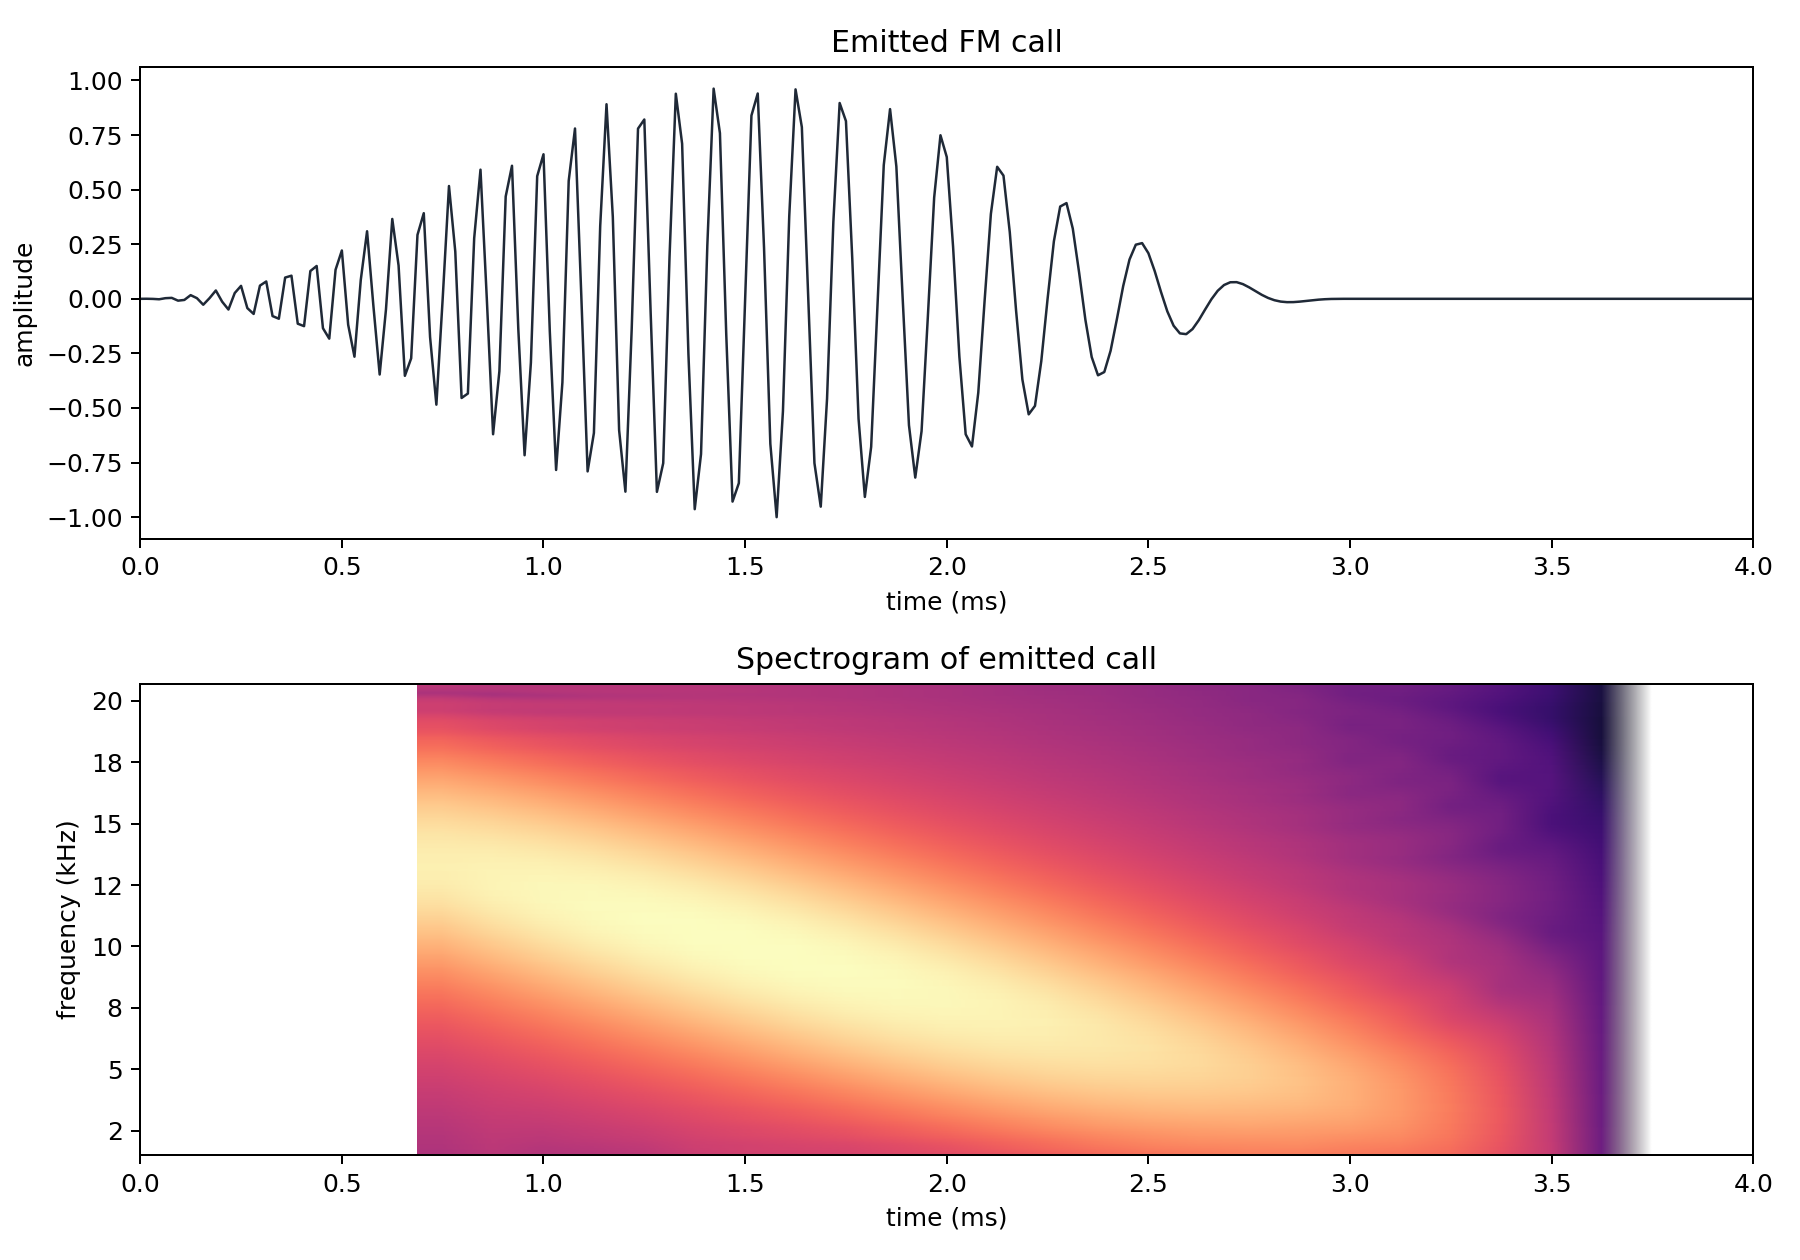
\includegraphics[width=\figwidth\linewidth]{ch1_emitted_call_spectrogram.png}
  \caption{The emitted frequency-modulated call used in the small-space experiments. The call sweeps downward through the cochlear band and provides multiple frequency-specific delay measurements.}
\end{figure}

\section{The Biomimetic Pivot}

Bats solve a related problem with limited biological hardware. They emit short frequency-modulated calls, receive echoes with two ears, and infer distance, azimuth, elevation, and object structure. The relevant lesson is not that an artificial system should copy every anatomical detail. Rather, the bat auditory system suggests an architecture: specialised parallel pathways extract timing, binaural level, and spectral-shape cues before later population-code integration.

This project therefore treats biology as a design prior. Each structure is interpreted functionally:
\begin{itemize}
  \item the cochlea is a frequency-selective sparse encoder;
  \item the VCN sharpens onset timing;
  \item the lateral lemniscus can suppress repeated or late responses;
  \item the IC provides coincidence and convergence;
  \item the SC or cortical readout can be modelled as a population-code decoder.
\end{itemize}

\begin{figure}[H]
  \centering
  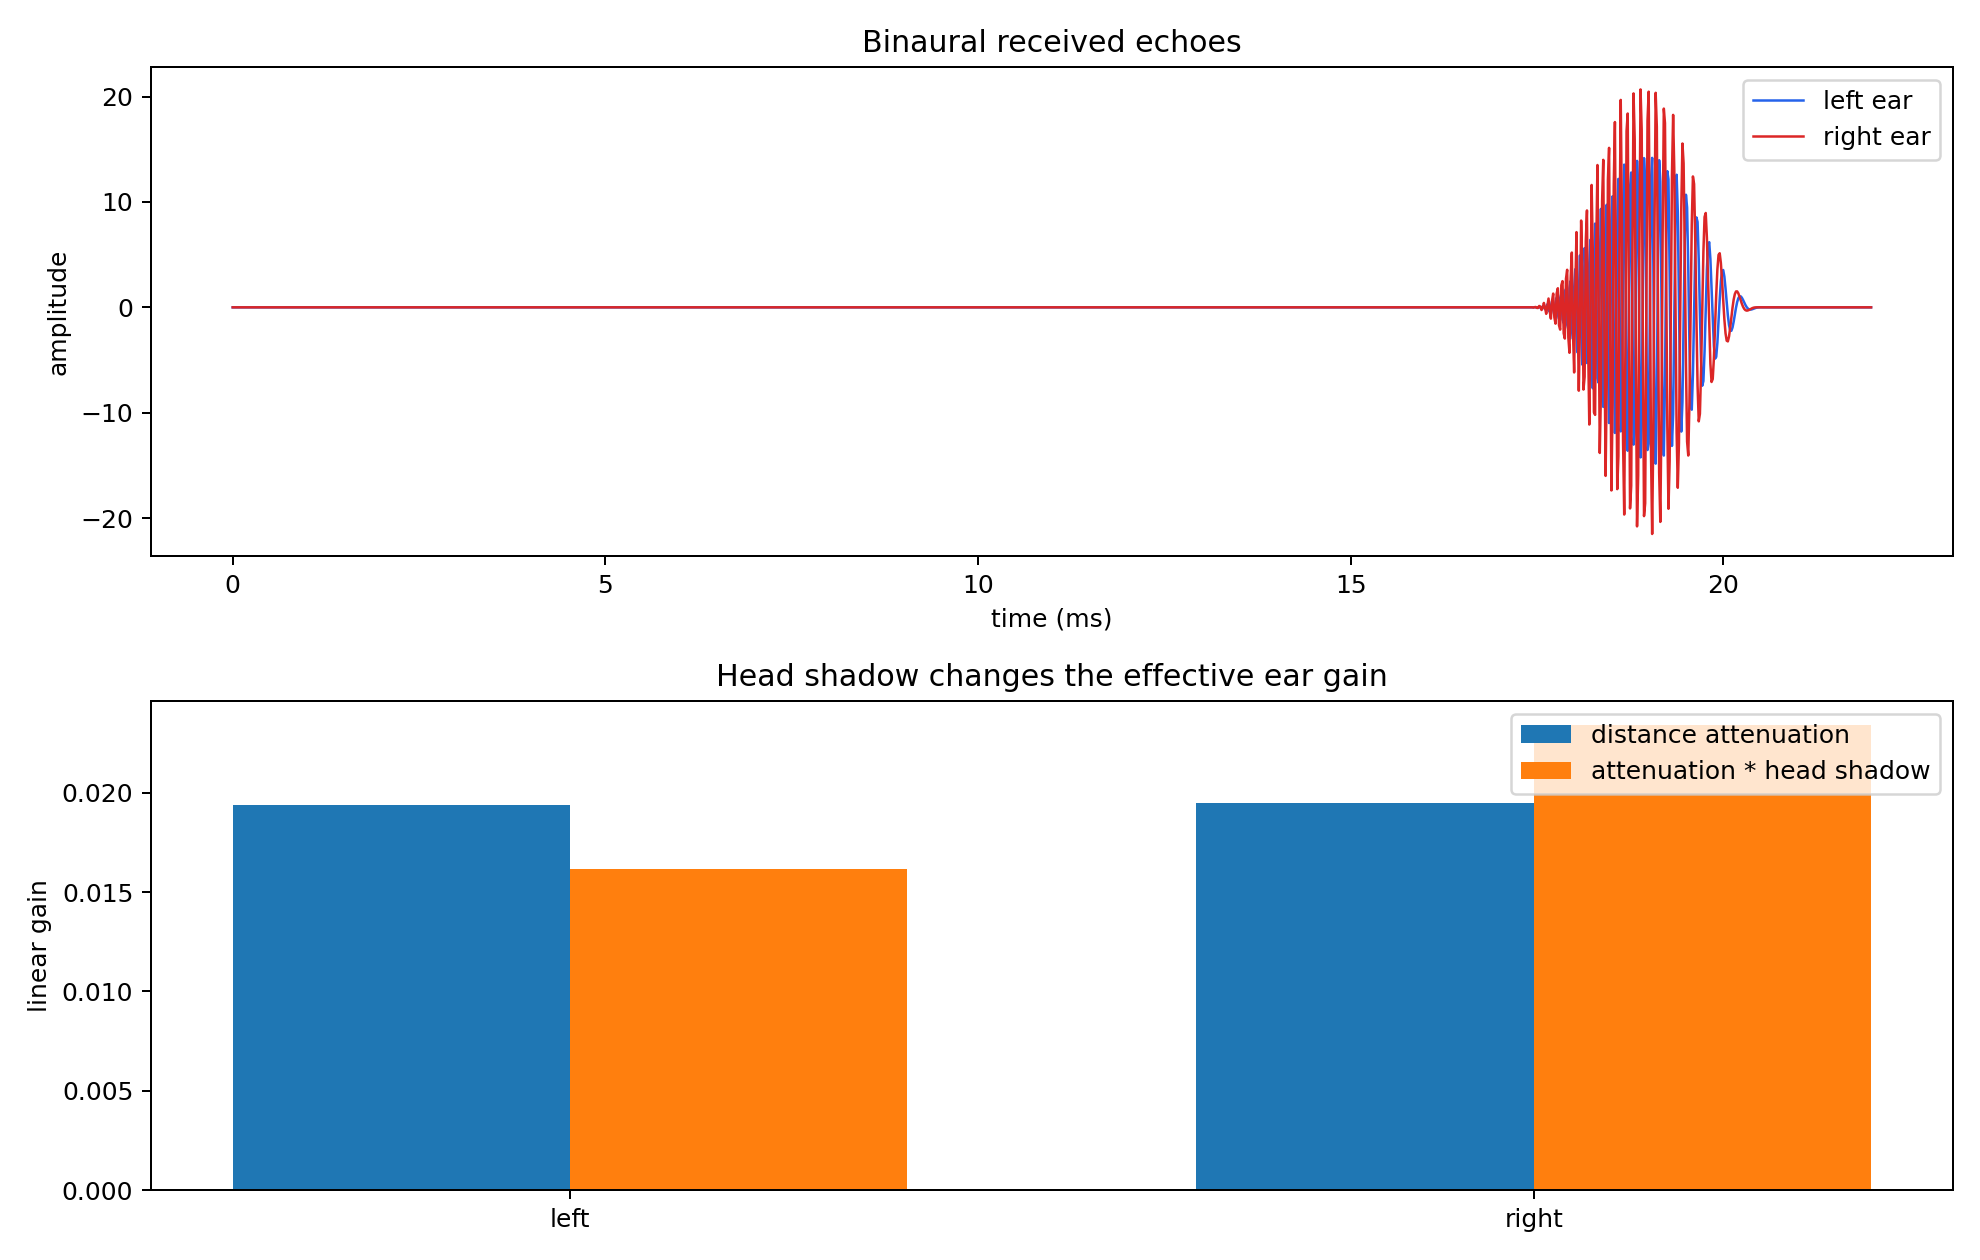
\includegraphics[width=\figwidth\linewidth]{ch1_binaural_head_shadow.png}
  \caption{Binaural amplitude differences caused by multiplicative head shadowing. This creates the main ILD cue used in the azimuth pathway.}
\end{figure}

\section{Architectural Philosophy}

The central methodological choice is bottom-up functional tuning rather than black-box end-to-end training. Earlier trained models showed that the features contain useful information: a fixed-feature ridge decoder achieved strong localisation performance. However, a trained decoder alone does not explain which cues are reliable or how to improve failures. The redesigned system therefore builds each cue pathway explicitly and tests it in isolation before integration.

This approach has three advantages. First, failures are interpretable. For example, noisy distance failures could be traced to cochlear noise spikes and onset detection. Second, computational cost can be assigned to a specific mechanism, such as IIR filtering or LIF spike generation. Third, later training can be targeted at modules where calibration is genuinely needed, instead of replacing the whole pipeline with an opaque network.

\chapter{Neuromorphic Primitives and Classical Algorithmic Parallels}

\section{Leaky Integrate-and-Fire Neurons}

The LIF neuron is the basic temporal accumulator used throughout the project. In discrete time it is written as
\[
  v_{t+1} = \beta v_t + I_t,
\]
\[
  z_t = \mathbb{1}[v_{t+1} \geq v_{\mathrm{th}}],
\]
\[
  v_{t+1} \leftarrow v_{t+1} - z_t v_{\mathrm{th}}.
\]
The state $v_t$ is the membrane potential, $\beta$ controls leakage, $I_t$ is the input current, and $z_t$ is the spike. With subtractive reset, strong input can generate repeated spikes without discarding all residual evidence.

Algorithmically, the LIF neuron acts like a causal low-pass filter followed by a threshold. It is therefore useful for coincidence detection, evidence accumulation, and squelching. It is less suitable when precise high-frequency structure must be preserved, because leakage integrates over time.

\begin{figure}[H]
  \centering
  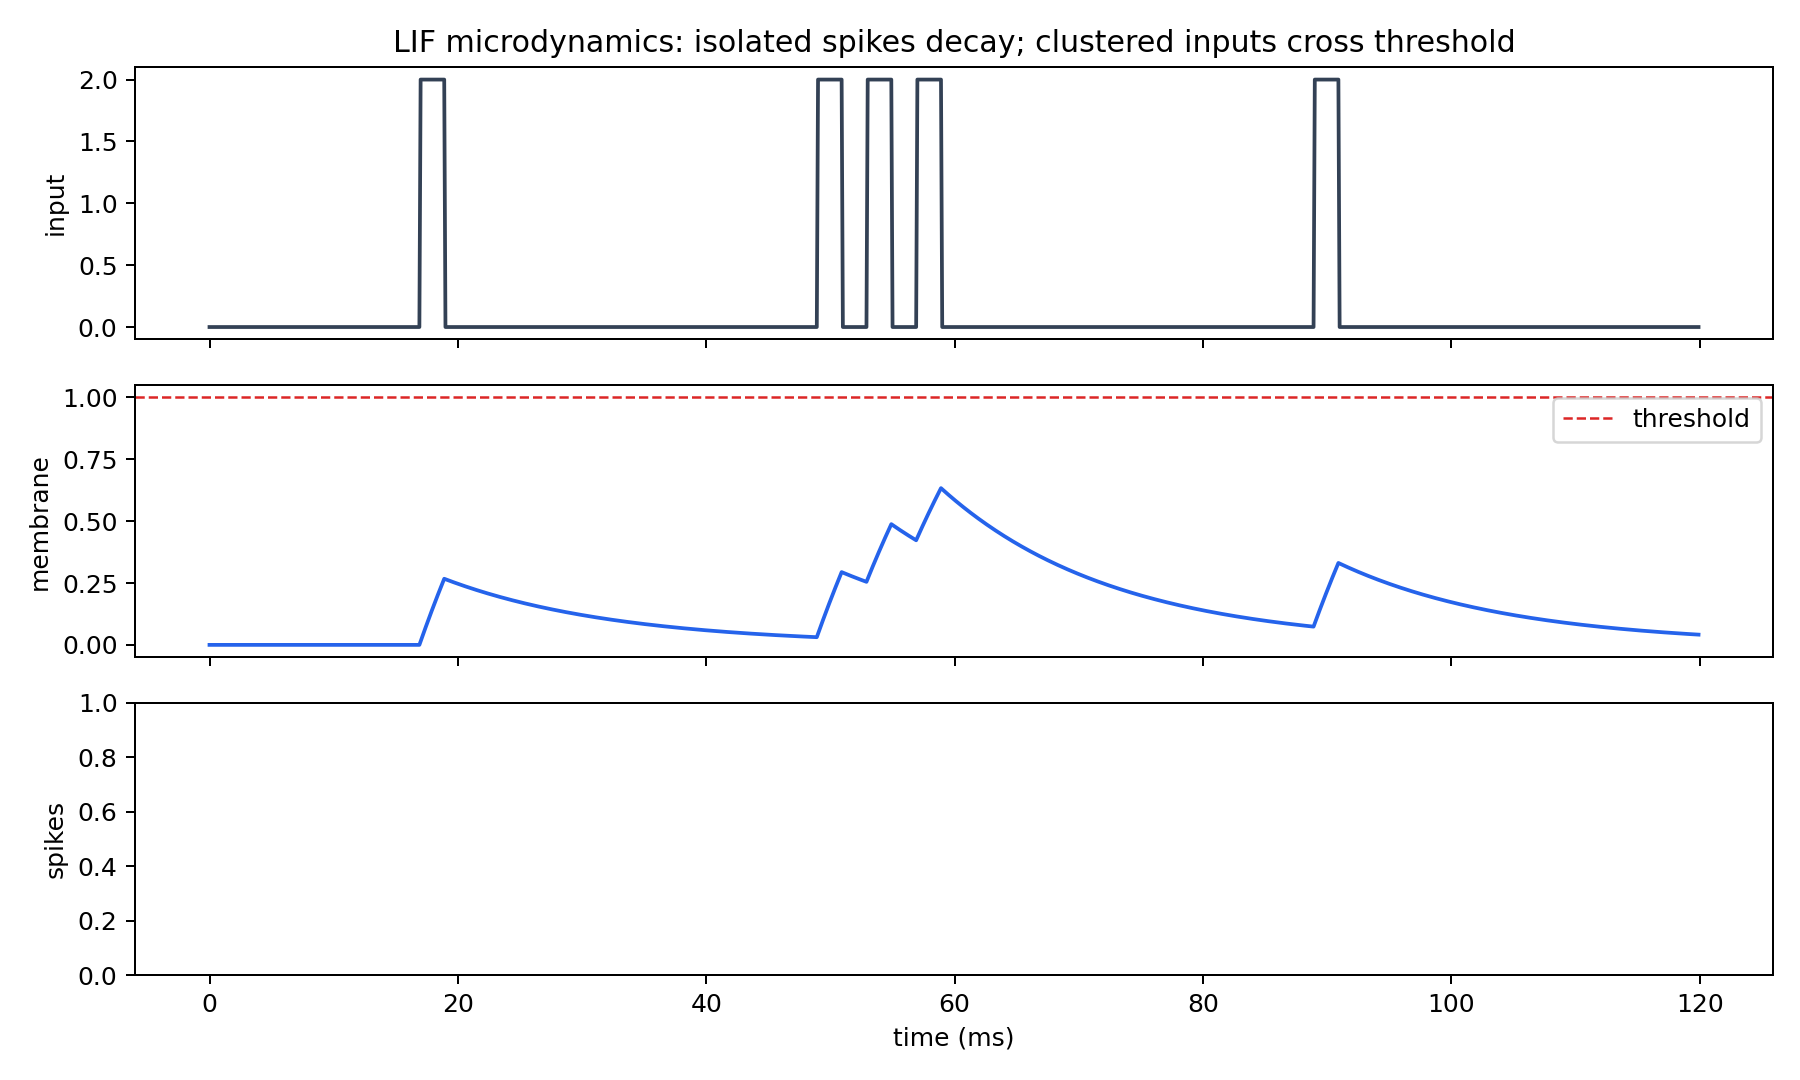
\includegraphics[width=\figwidth\linewidth]{ch2_lif_microdynamics.png}
  \caption{Micro-temporal LIF dynamics. Closely spaced inputs accumulate and cross threshold, while isolated inputs decay.}
\end{figure}

\section{Resonate-and-Fire Neurons}

The resonate-and-fire (RF) neuron is a second-order oscillator with a spiking threshold. A simplified discrete update is
\[
  u_{t+1} = \rho u_t + g I_t - \omega x_t,
\]
\[
  x_{t+1} = x_t + \omega u_{t+1},
\]
\[
  z_t = \mathbb{1}[x_{t+1} \geq \vartheta],
\]
where $x_t$ is the resonant state, $u_t$ is an auxiliary state analogous to velocity or imaginary voltage, $\rho$ is damping, and $\omega$ is the resonant frequency parameter. The RF neuron is therefore a band-pass primitive.

\begin{figure}[H]
  \centering
  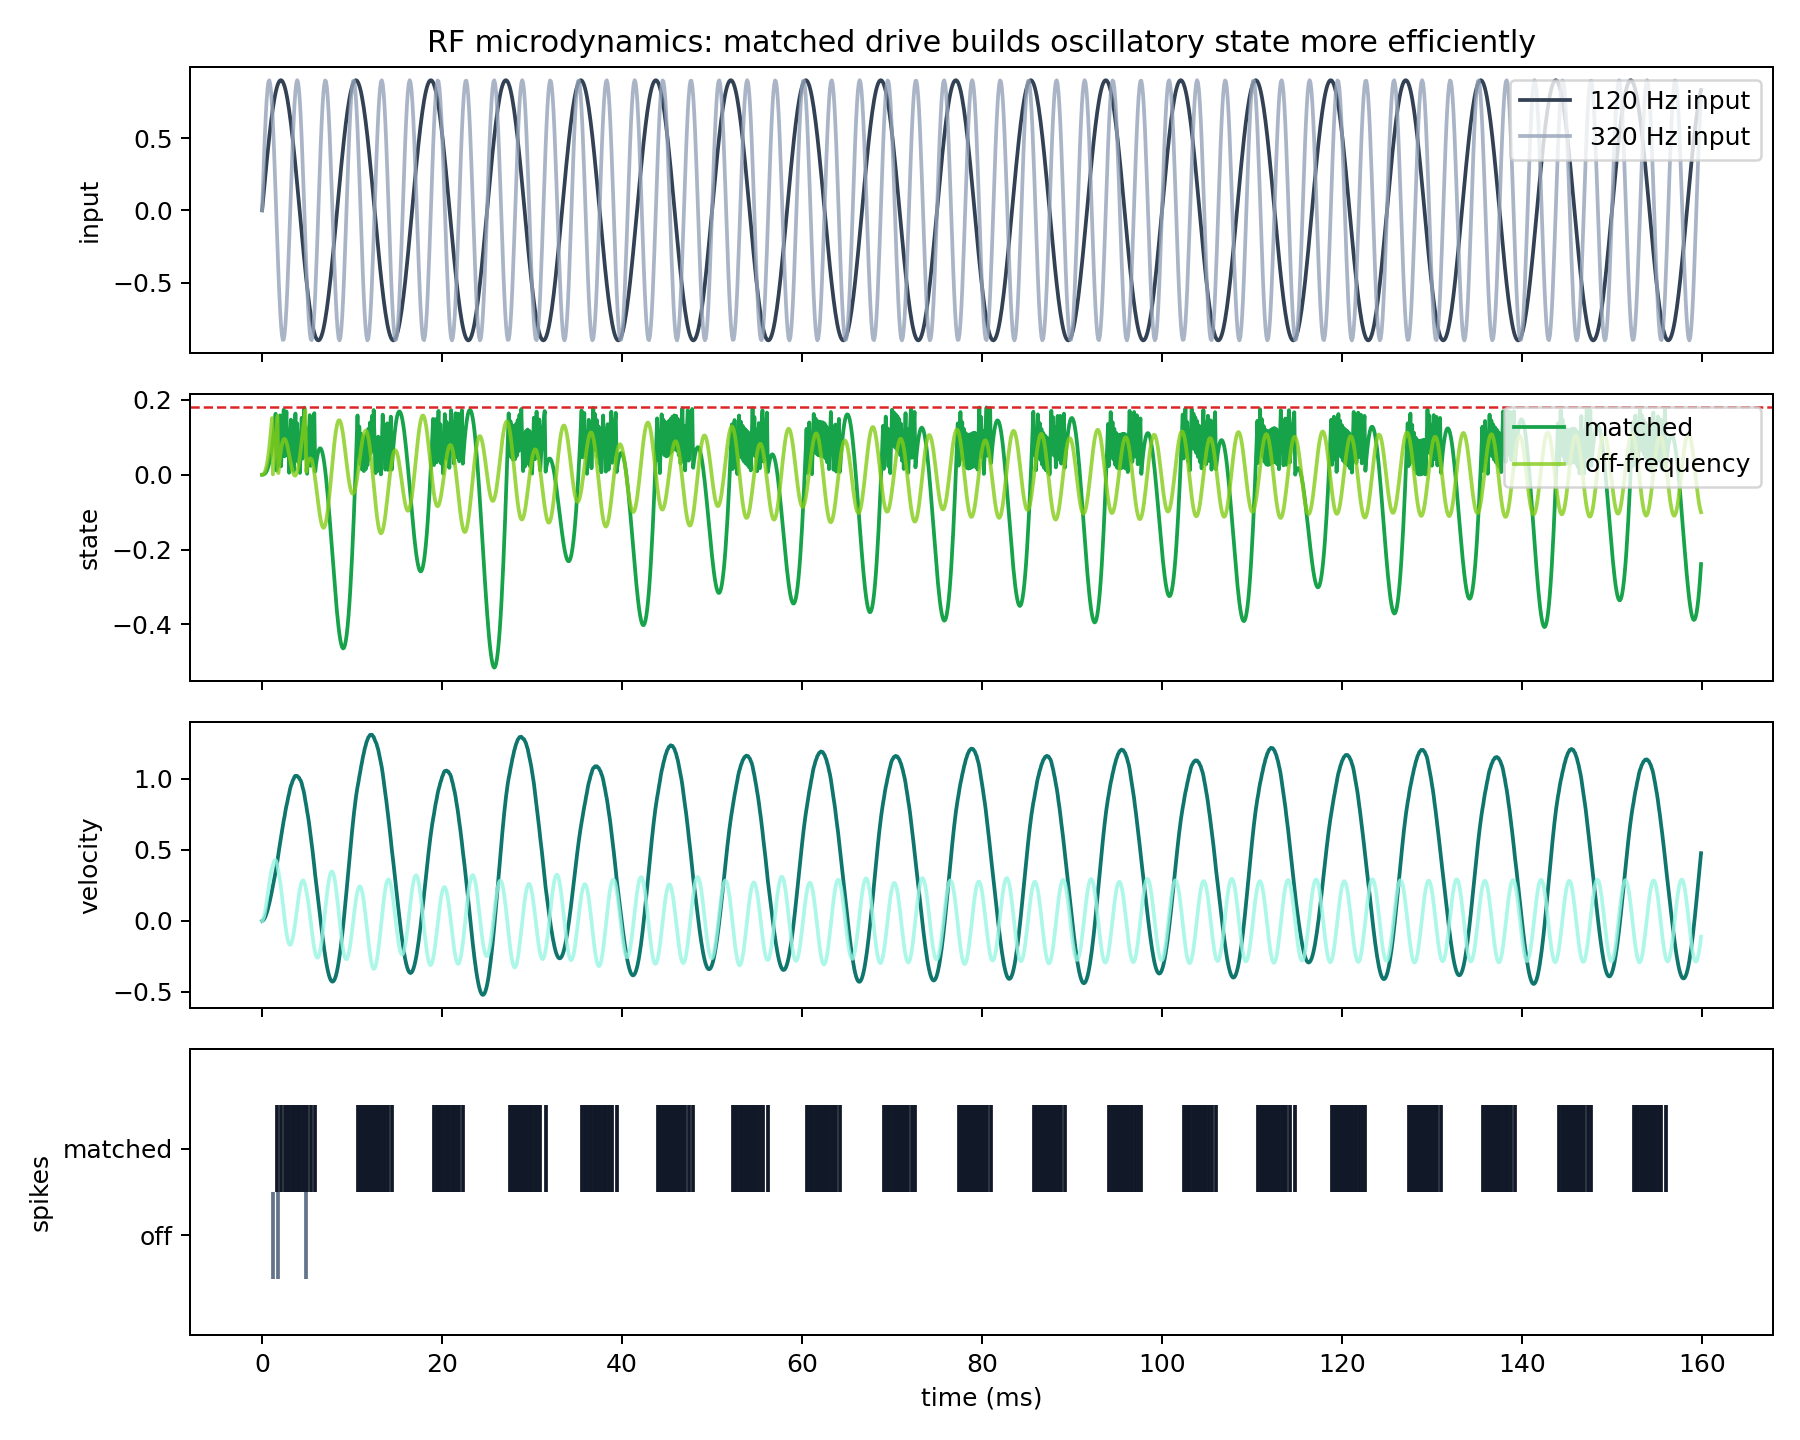
\includegraphics[width=\figwidth\linewidth]{ch2_rf_microdynamics.png}
  \caption{Micro-temporal RF dynamics. The oscillatory state builds most strongly when input timing matches the resonant mode.}
\end{figure}

\section{Level-Crossing Encoding}

A level-crossing encoder emits events when a signal changes by a specified amount. For reference level $q_t$ and signal $x_t$,
\[
  z_t^{+} = \mathbb{1}[x_t - q_t \geq \Delta],
\]
\[
  z_t^{-} = \mathbb{1}[q_t - x_t \geq \Delta].
\]
After an up or down event the reference is moved by $\Delta$. This encodes change rather than absolute level. It is attractive for event-based processing, but it is sensitive to the chosen step size and does not preserve amplitude unless multiple thresholds or adaptation are used.

\section{Neurons as Algorithms}

The project repeatedly uses the idea that a biological circuit can be interpreted as an algorithmic primitive. The mapping is not exact, but it is useful for design.

\begin{table}[H]
  \centering
  \caption{Functional parallels between neuromorphic primitives and classical algorithms.}
  \begin{tabular}{lll}
    \toprule
    Neuromorphic structure & Algorithmic analogue & Project use\\
    \midrule
    Cochlear filterbank & Filterbank / short-time spectrum & Frequency decomposition\\
    LIF neuron & Leaky integrator + threshold & Onset and coincidence evidence\\
    RF neuron & Band-pass resonator & Frequency-selective detection\\
    Delay-line coincidence & Cross-correlation & Range and ITD estimation\\
    Synaptic weight template & Matched filter & Elevation notch detection\\
    Population spikes & Sampled posterior-like code & SC readout\\
    CANN recurrence & Smoothing prior / attractor dynamics & Stabilised spatial map\\
    \bottomrule
  \end{tabular}
\end{table}

\section{Preliminary Primitive Experiments}

The neuron analysis showed that the LIF response behaves as a low-pass accumulator, while the RF response is frequency selective. The RF neuron can produce a sharper-looking response, but this did not automatically improve distance accuracy in the early coincidence experiments. The reason is that localisation accuracy depends on whether the peak of the response map falls into the correct delay bin, not only on whether the response looks visually sharp. RF detectors are more sensitive to tuning mismatch and repeated input structure, whereas LIF coincidence detectors are more forgiving for single-pulse delay estimation.

\begin{figure}[H]
  \centering
  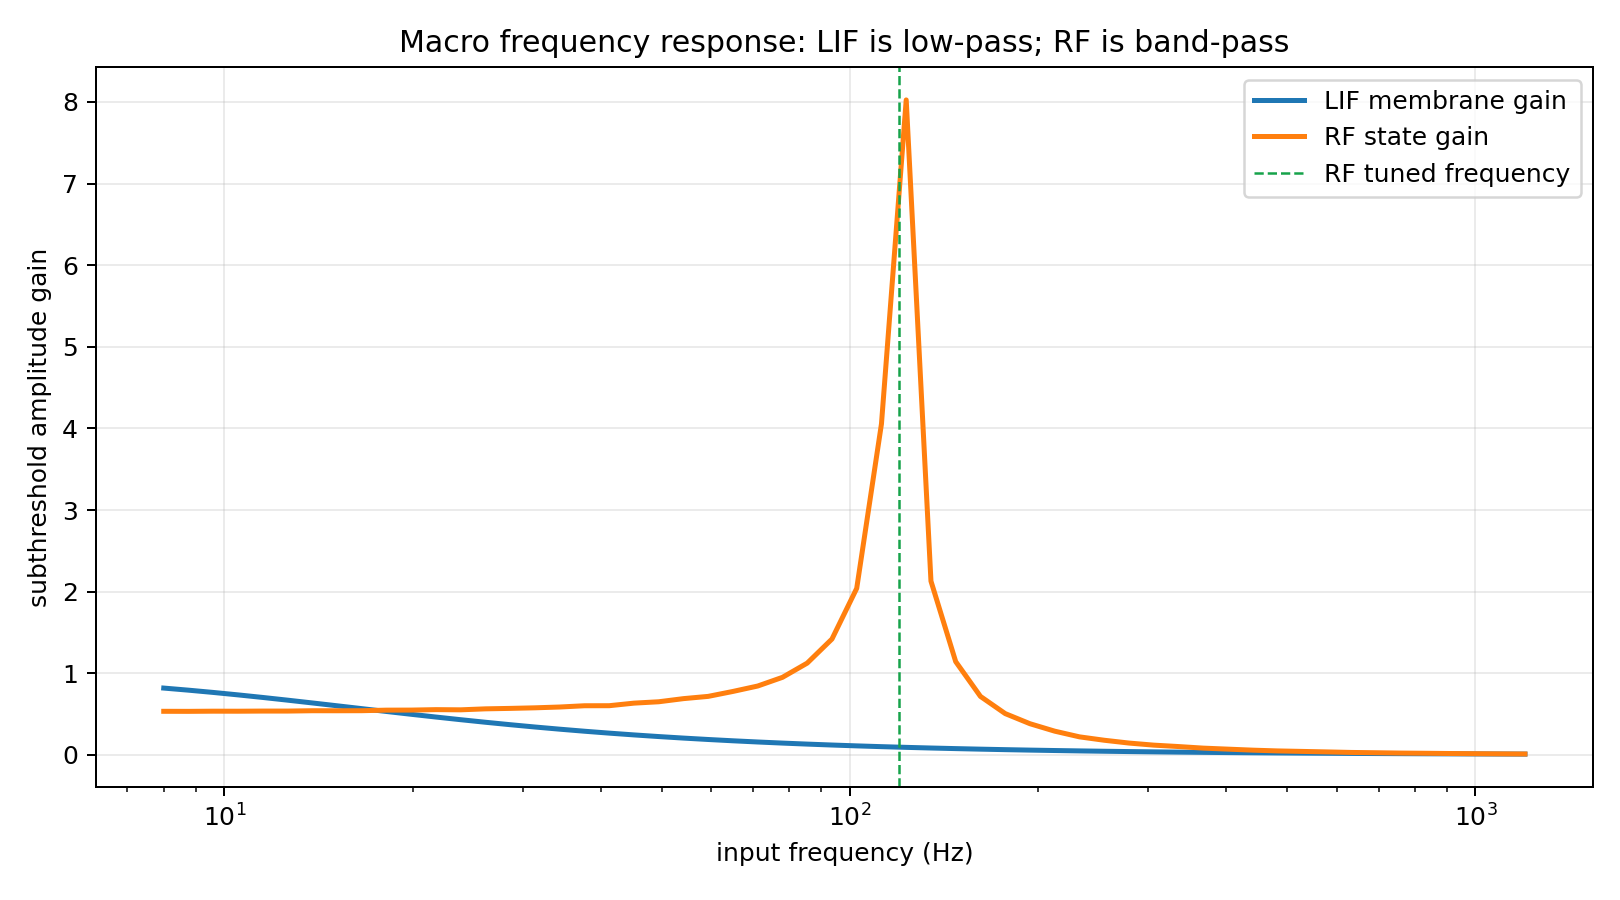
\includegraphics[width=\figwidth\linewidth]{ch2_frequency_gain.png}
  \caption{Macro frequency response of the LIF, RF, and level-crossing primitives. The LIF behaves as a low-pass accumulator, while the RF neuron peaks near its resonance.}
\end{figure}

\begin{figure}[H]
  \centering
  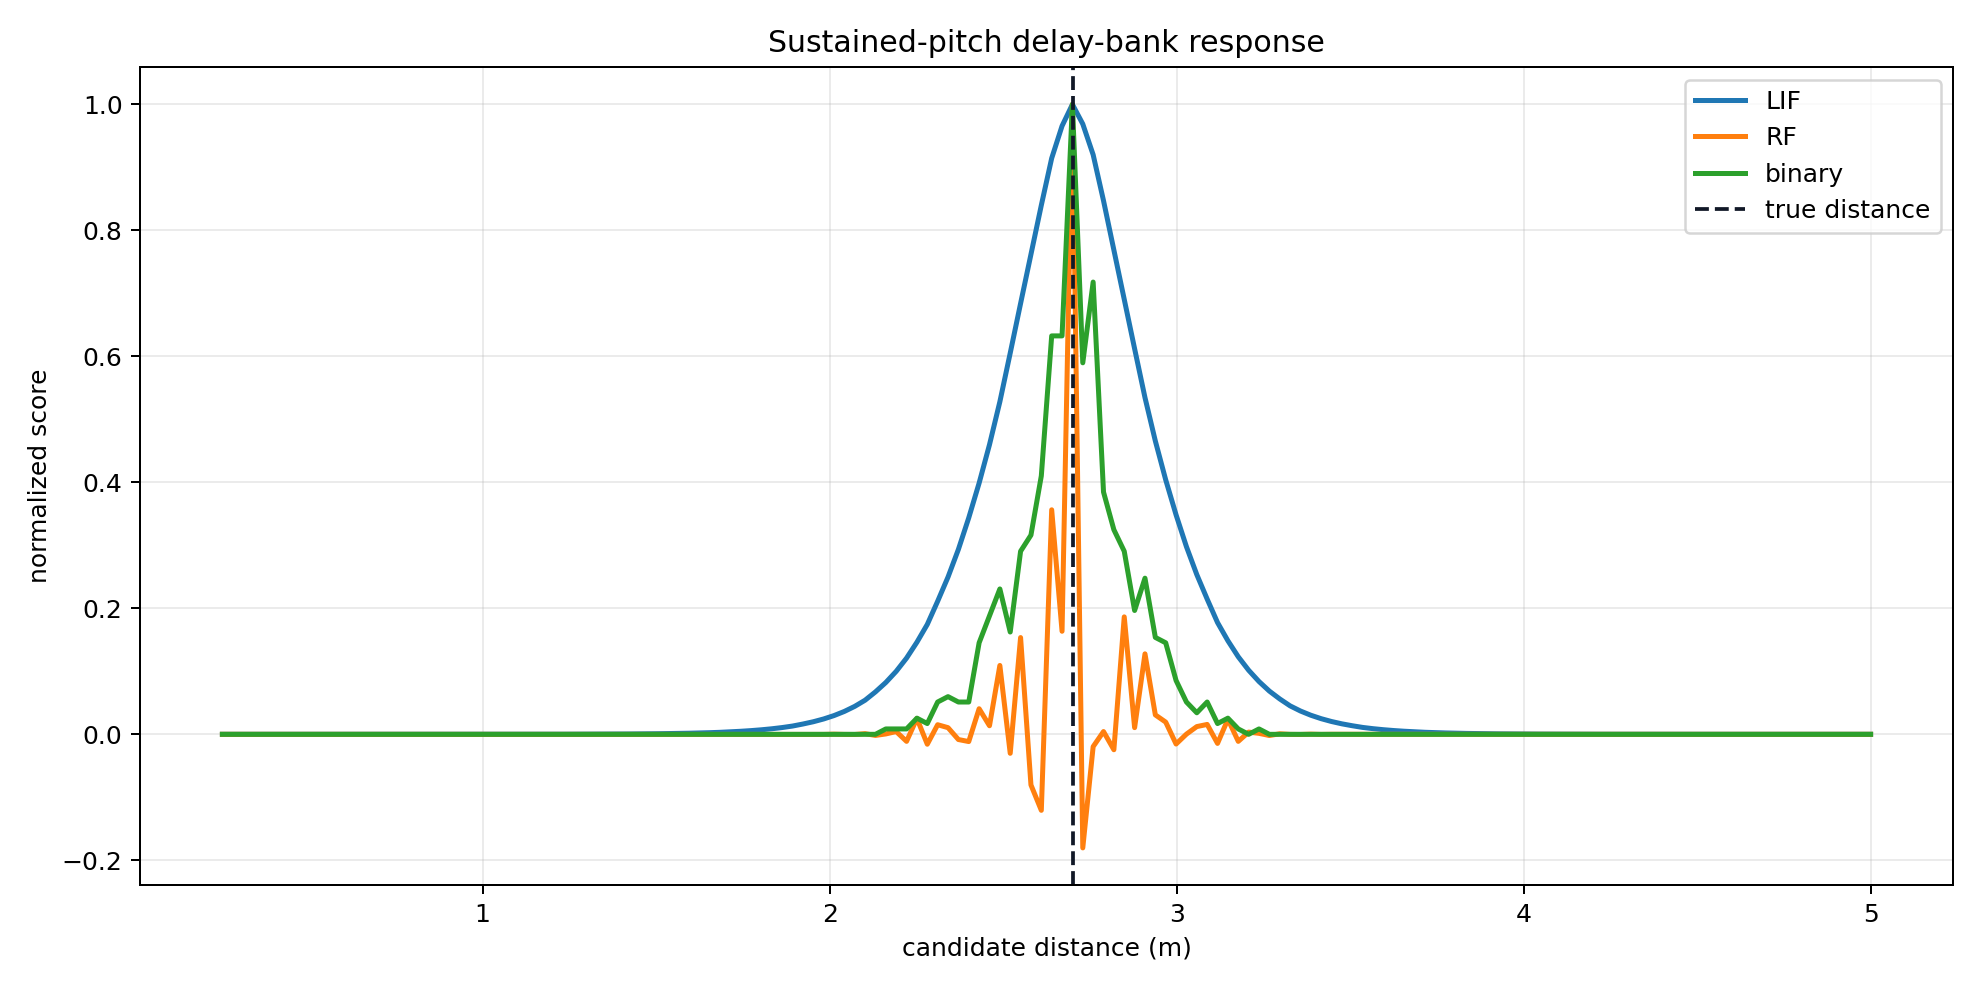
\includegraphics[width=\figwidth\linewidth]{ch2_sustained_pitch_response.png}
  \caption{Sustained spiking-input test. Repeated structured inputs reduce noise sensitivity, but they also show that RF accuracy depends strongly on matching the stimulus statistics.}
\end{figure}

\chapter{System Architecture and Peripheral Frontend}

\section{Acoustic Signal Model}

The emitted call is a Hann-windowed linear frequency-modulated chirp,
\[
  s(t) = A w(t) \sin\left(2\pi\left[f_0 t + \frac{k}{2}t^2\right]\right),
\]
where $w(t)$ is the Hann window and $k=(f_1-f_0)/T$ is the chirp slope. In the main small-space experiments the call sweeps from 18 kHz down to 2 kHz over 3 ms at a 64 kHz sample rate. Later tests use the active call band above 4 kHz for robust distance processing.

For a target at range $r$, the first-order echo delay is approximately
\[
  \tau = \frac{2r}{c},
\]
with binaural corrections from the different path lengths to the two ears. The received amplitude is modelled as
\[
  A_{\mathrm{echo}} = \frac{0.7}{L^2},
\]
where $L$ is the full acoustic path length. This factor is not a complete physical room-acoustics model; it is an engineered free-field attenuation convention used consistently across the simulations.

\section{Cochlea Model}

The final cochlea model uses a bank of IIR filters rather than the original FFT/IFFT filterbank. Each frequency channel is a stable second-order resonator. A convenient form is
\[
  y_c[t] = b_{0,c}x[t] + b_{1,c}x[t-1] + b_{2,c}x[t-2]
          - a_{1,c}y_c[t-1] - a_{2,c}y_c[t-2].
\]
Stability requires the poles to lie inside the unit circle. In the tuned model, the resonator quality factor was increased to improve frequency selectivity while keeping the response stable.

The final optimised implementation combined IIR filtering, active-window gating, and a scripted LIF spike encoder. The active window avoids processing long silent regions, while the LIF encoder transforms the channel envelope into sparse spikes.

\begin{figure}[H]
  \centering
  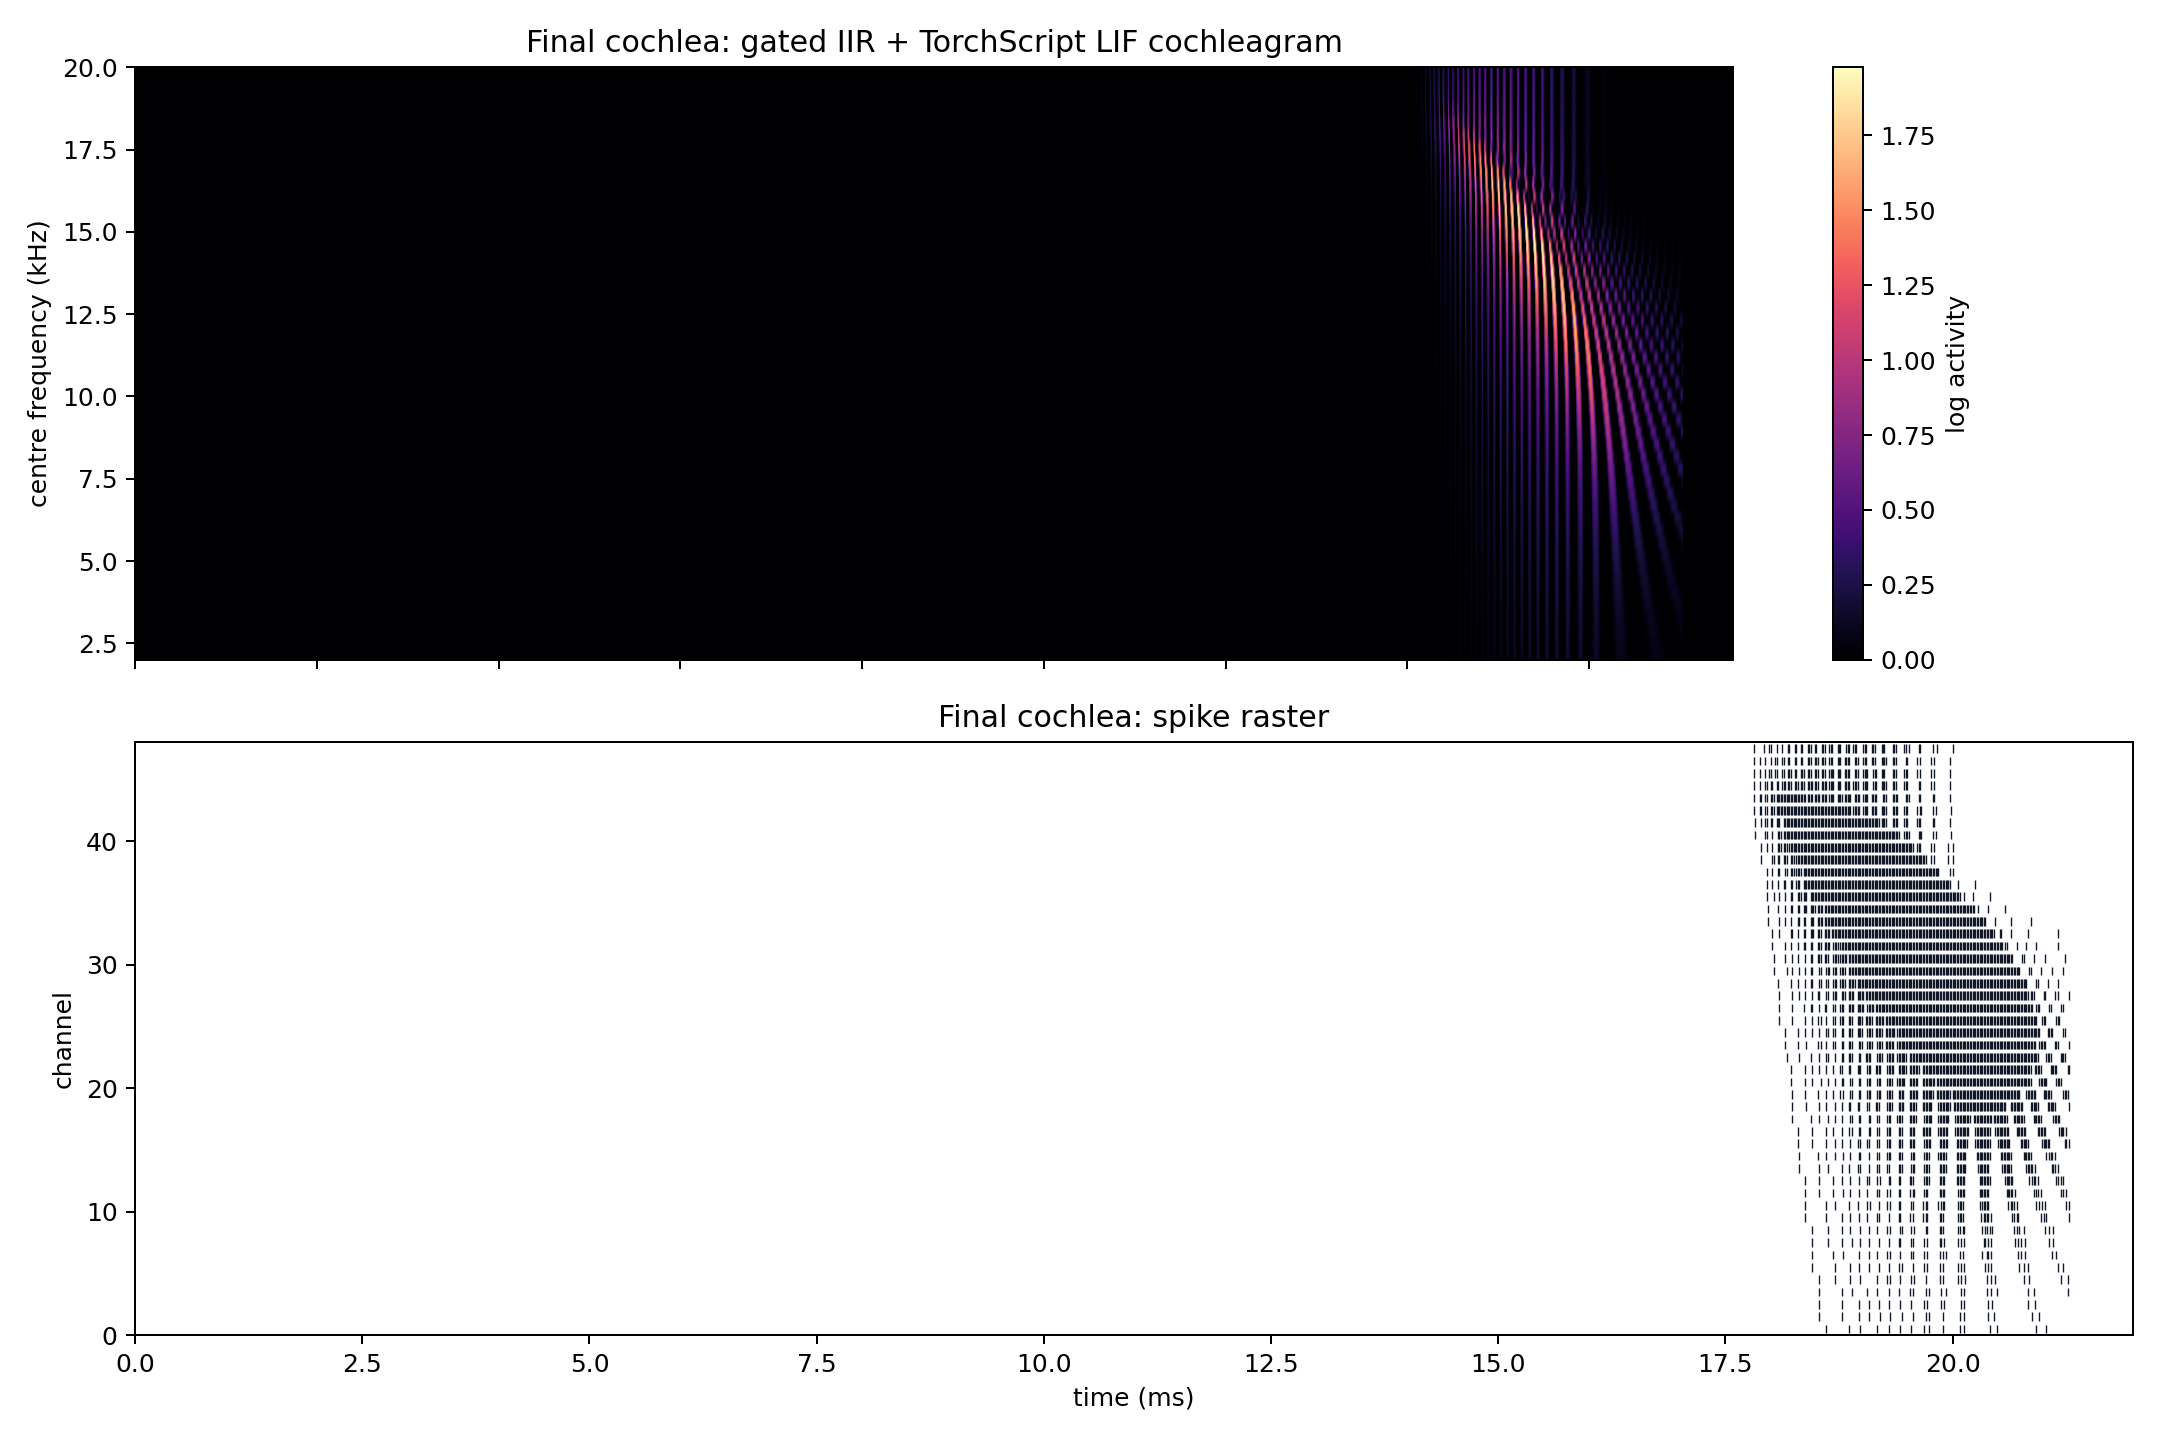
\includegraphics[width=\figwidth\linewidth]{ch3_final_cochlea_output.png}
  \caption{Final cochlea output for the optimised IIR + LIF model. The cochleagram and spike raster show the emitted sweep after frequency-selective filtering and sparse encoding.}
\end{figure}

\section{Runtime Scaling}

The IIR cochlea was selected because it scales more favourably with channel count than the old FFT/IFFT approach in the tested regime. At 48 channels the final IIR model required approximately 2.9--3.3 ms per signal depending on timing conditions, while the FFT model was approximately 5.1 ms. At 1000 channels the final IIR model was approximately 10.7 ms, compared with approximately 53.2 ms for the FFT model. This supports the use of the IIR model for later pathway experiments.

\begin{figure}[H]
  \centering
  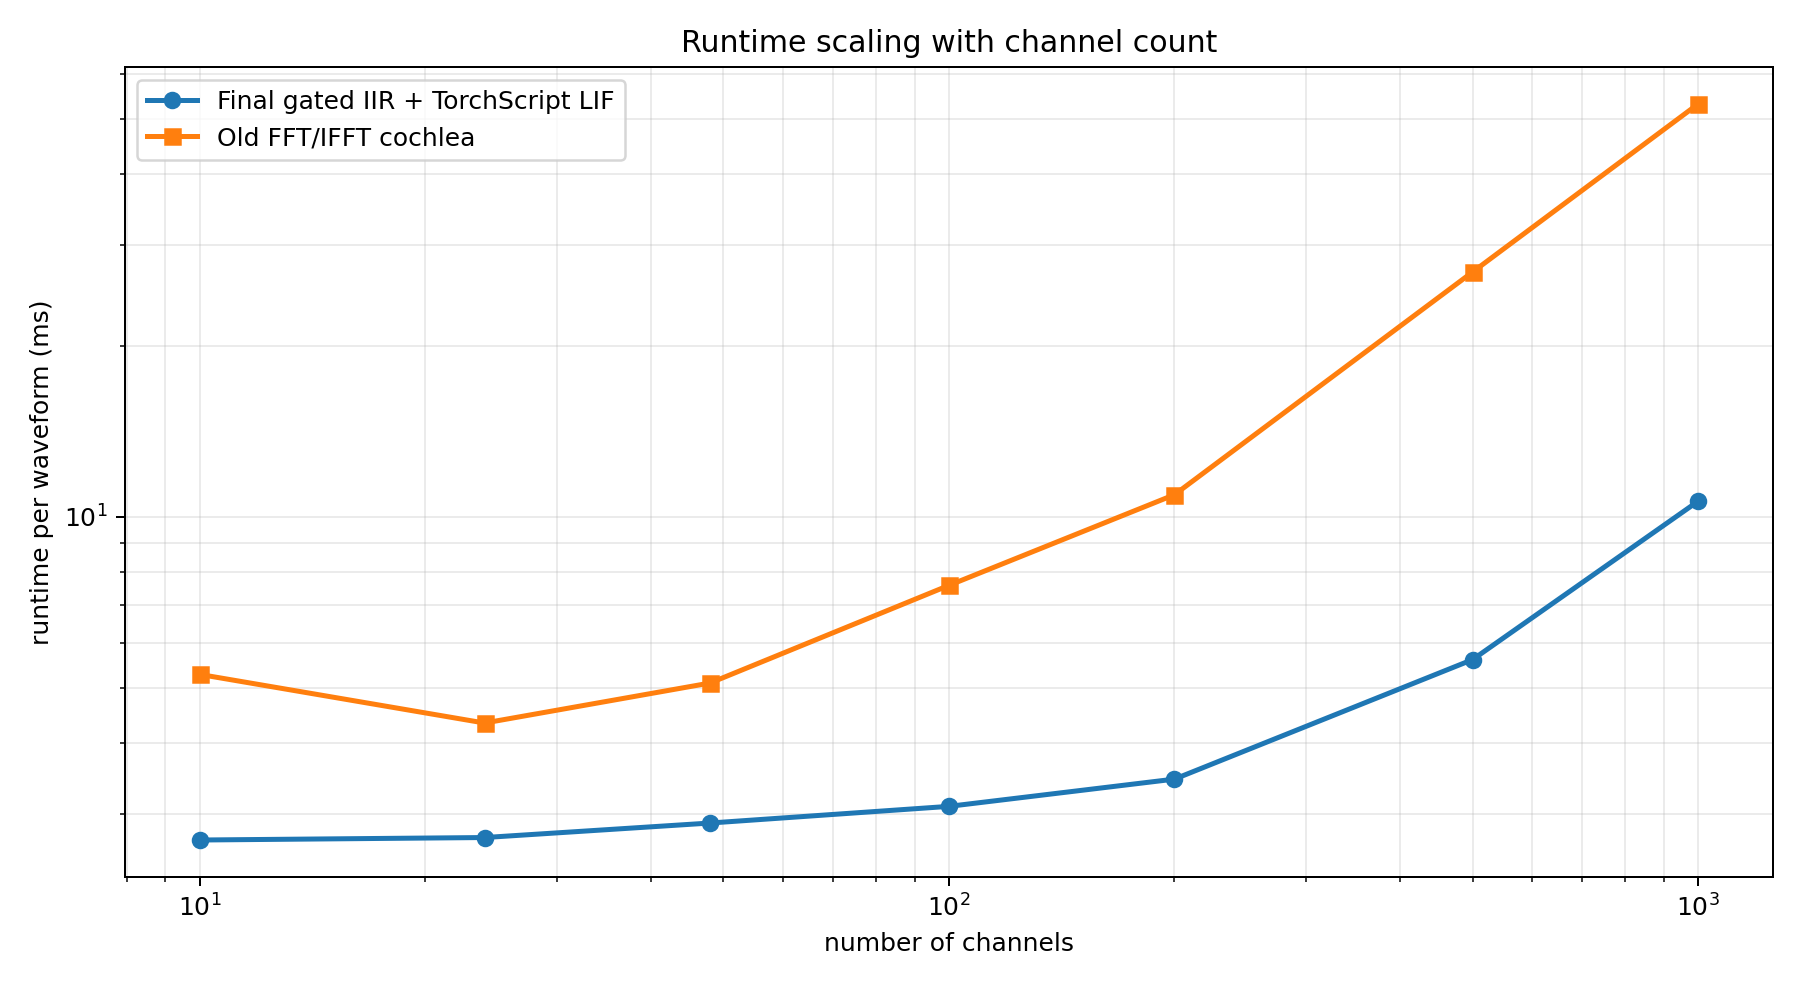
\includegraphics[width=\figwidth\linewidth]{ch3_channel_scaling_runtime.png}
  \caption{Measured runtime as the number of cochlear channels is increased. The IIR model is preferable for the channel counts considered in this project.}
\end{figure}

\section{Dynamic Squelch Frontend}

A fixed cochlear threshold creates an amplitude-latency trap. If the threshold is low enough to detect weak distant echoes, early noise can trigger false spikes. If it is high enough to suppress early noise, distant echoes can disappear. The final distance pathway therefore uses a dynamic threshold and leak:
\[
  v_{\mathrm{th}}(t) = v_{\infty} + (v_0 - v_{\infty})e^{-t/\tau_{\theta}},
\]
\[
  \beta(t) = \beta_{\infty} - (\beta_{\infty} - \beta_0)e^{-t/\tau_{\beta}}.
\]
The selected version used a threshold decay from 16 to 2.5 and a beta increase from 0.2 to 0.6. Channels below 4 kHz were silenced for distance processing because the call of interest does not use those frequencies.

\begin{figure}[H]
  \centering
  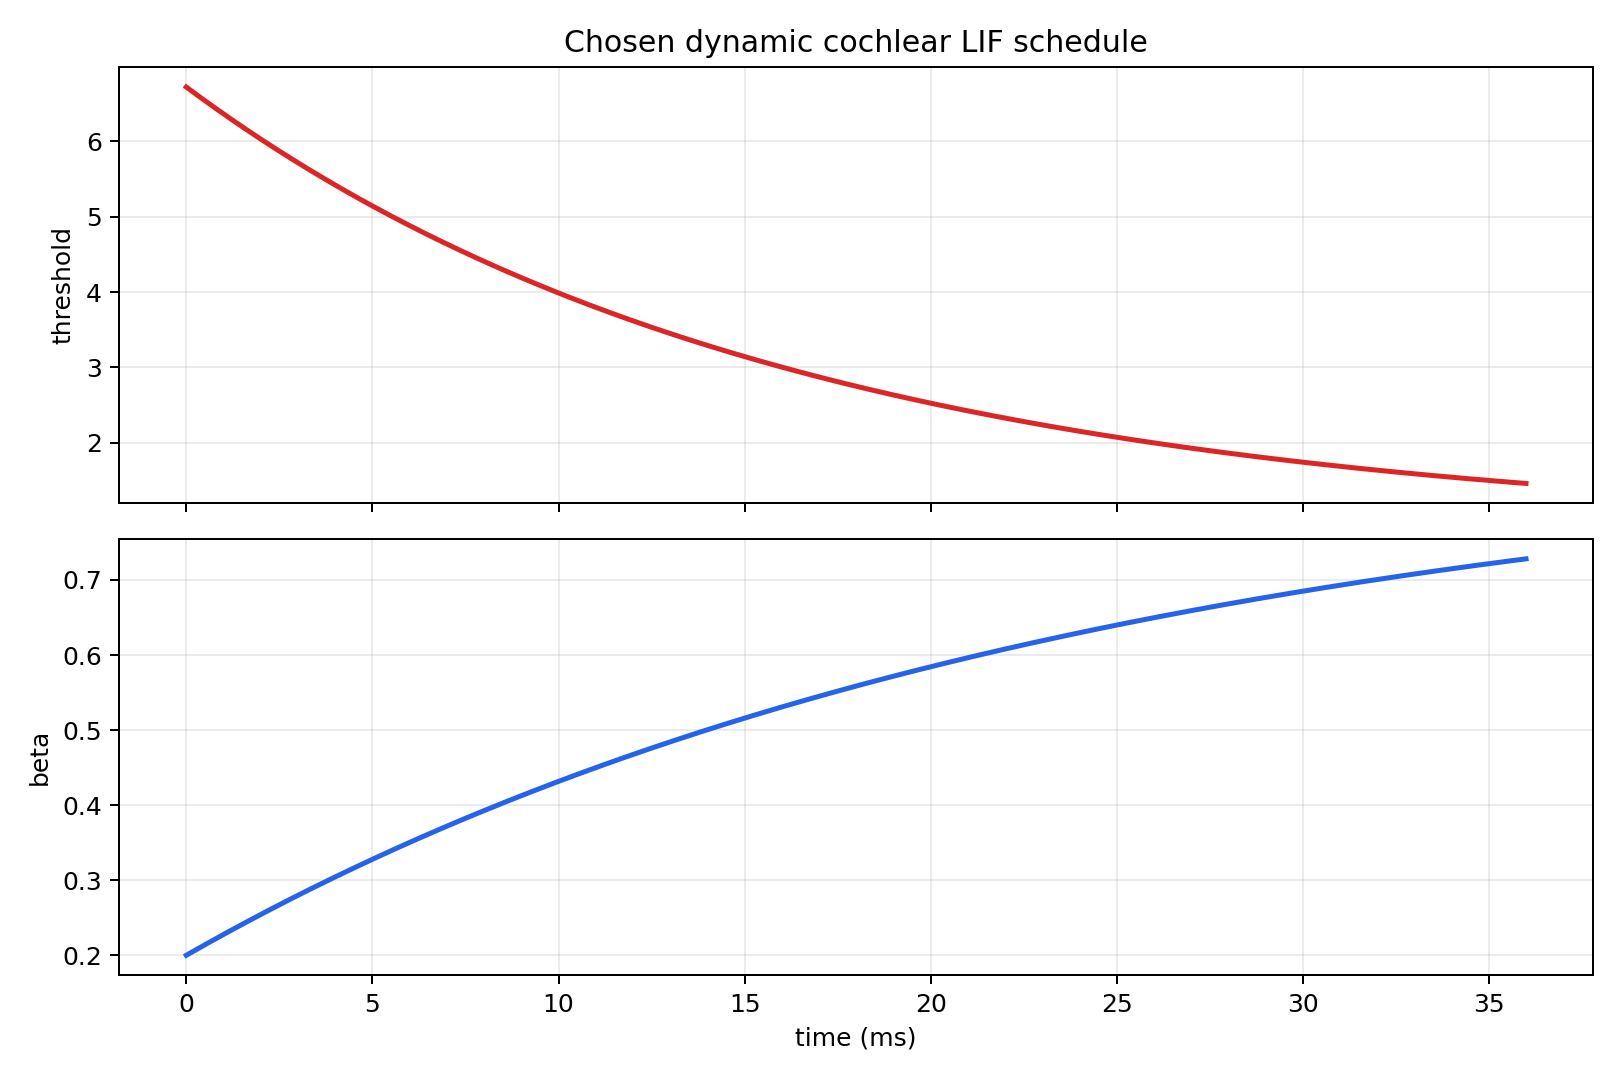
\includegraphics[width=\figwidth\linewidth]{ch3_dynamic_schedule.png}
  \caption{Dynamic threshold and beta schedule used by the robust cochlear frontend. The threshold relaxes with time while the membrane becomes more integrative.}
\end{figure}

\section{VCN Onset Calibration}

The VCN stage sharpens the cochlear output into onset spikes. A low-threshold, long-refractory LIF model was compared against a simpler first-spike detector. The LIF onset model was more stable because it integrates across small local fluctuations before firing, whereas a first-spike rule can be triggered by isolated noise or filter leakage. A latency vector was calibrated and then applied to the corollary discharge, not subtracted from the echo, preserving causality.

\begin{figure}[H]
  \centering
  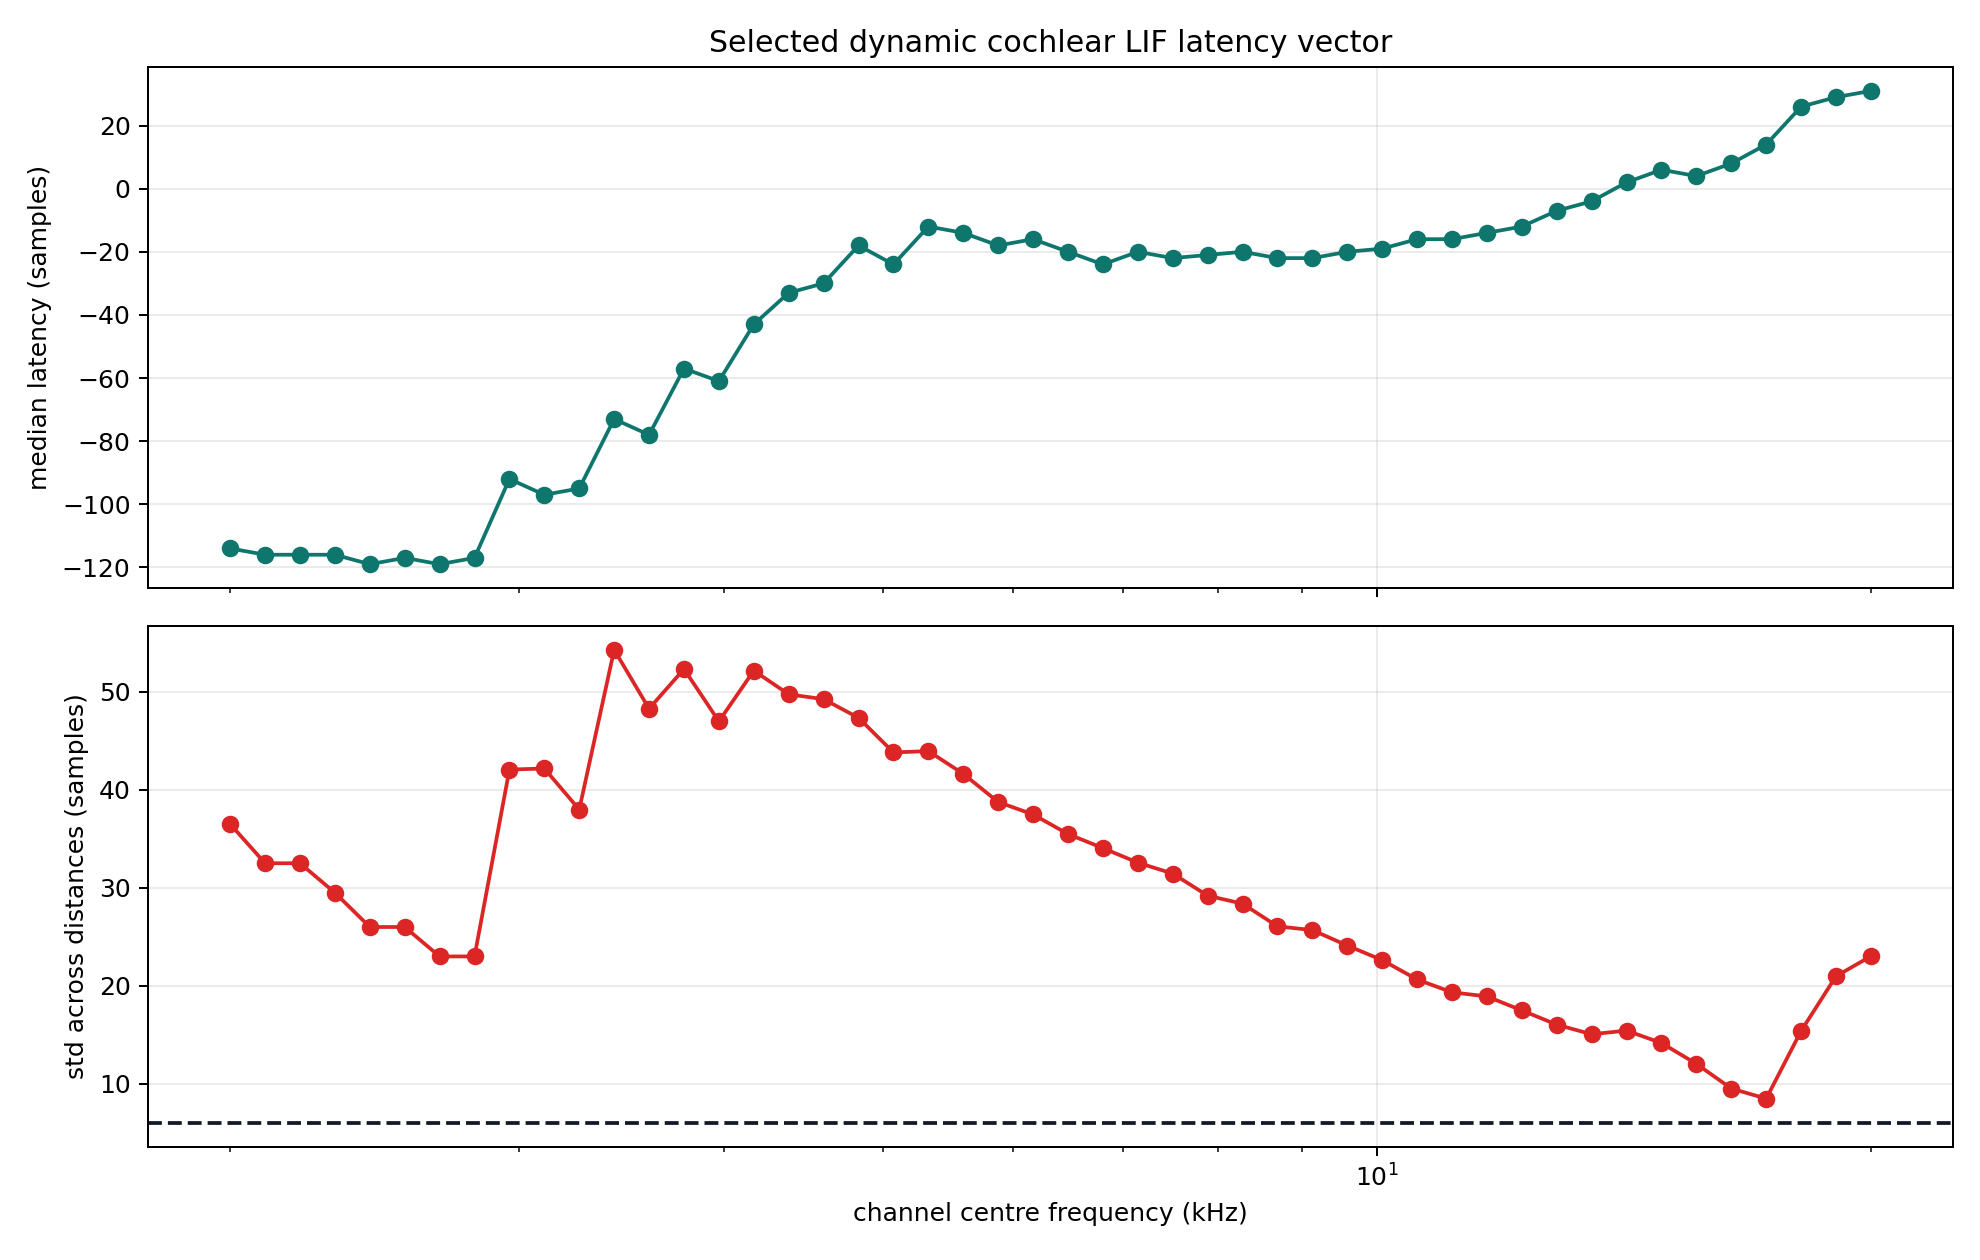
\includegraphics[width=\figwidth\linewidth]{ch3_cochlea_latency_vector.png}
  \caption{Cochlear latency vector used to align the expected corollary discharge sweep with the measured onset timing of each frequency channel.}
\end{figure}

\chapter{Parallel Processing Pathways}

\section{Distance Pathway}

\subsection{Biological Mechanism}

Distance in echolocation is primarily a temporal problem. A bat emits a call and receives an echo after a delay proportional to range. The biological auditory system contains several structures that sharpen timing and create coincidence-like responses. In the model these are abstracted as a cochlea, VCN onset detector, DNLL-style suppression, IC coincidence detector, AC topographic map, and SC readout.

\begin{figure}[H]
  \centering
  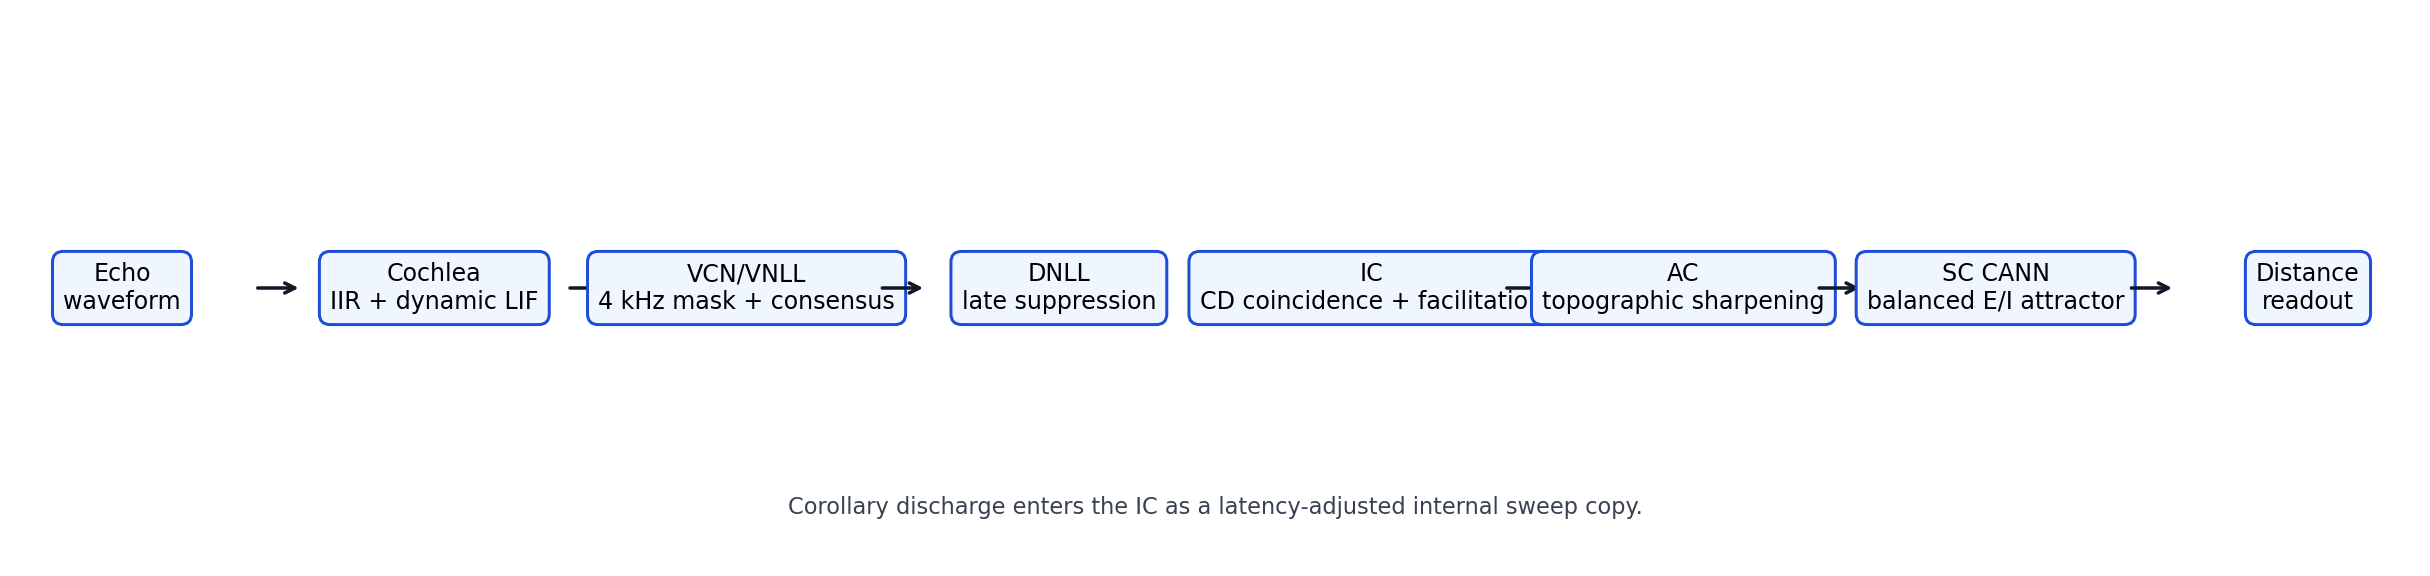
\includegraphics[width=\figwidth\linewidth]{ch4_distance_pipeline.png}
  \caption{Final distance pathway structure. The pathway transforms cochlear spikes into onset events, compares them with a corollary discharge, organises the result into a distance map, and decodes range.}
\end{figure}

\subsection{Neuromorphic Abstraction}

For each candidate delay $d_k$, the IC computes a coincidence score between the VCN echo spike train $S_{\mathrm{VCN}}[c,t]$ and the corollary discharge $S_{\mathrm{CD}}[c,t]$:
\[
  C[k] = \sum_c \sum_t S_{\mathrm{VCN}}[c,t] S_{\mathrm{CD}}[c,t-d_k].
\]
The candidate delay grid maps to distance through
\[
  r_k = \frac{c d_k \Delta t}{2}.
\]
The AC applies lateral sharpening with a Mexican-hat-like kernel, and the simplest SC readout computes a centre of mass:
\[
  \hat{r} = \frac{\sum_k r_k a_k}{\sum_k a_k + \epsilon},
\]
where $a_k$ is the final activation of distance bin $k$.

\begin{figure}[H]
  \centering
  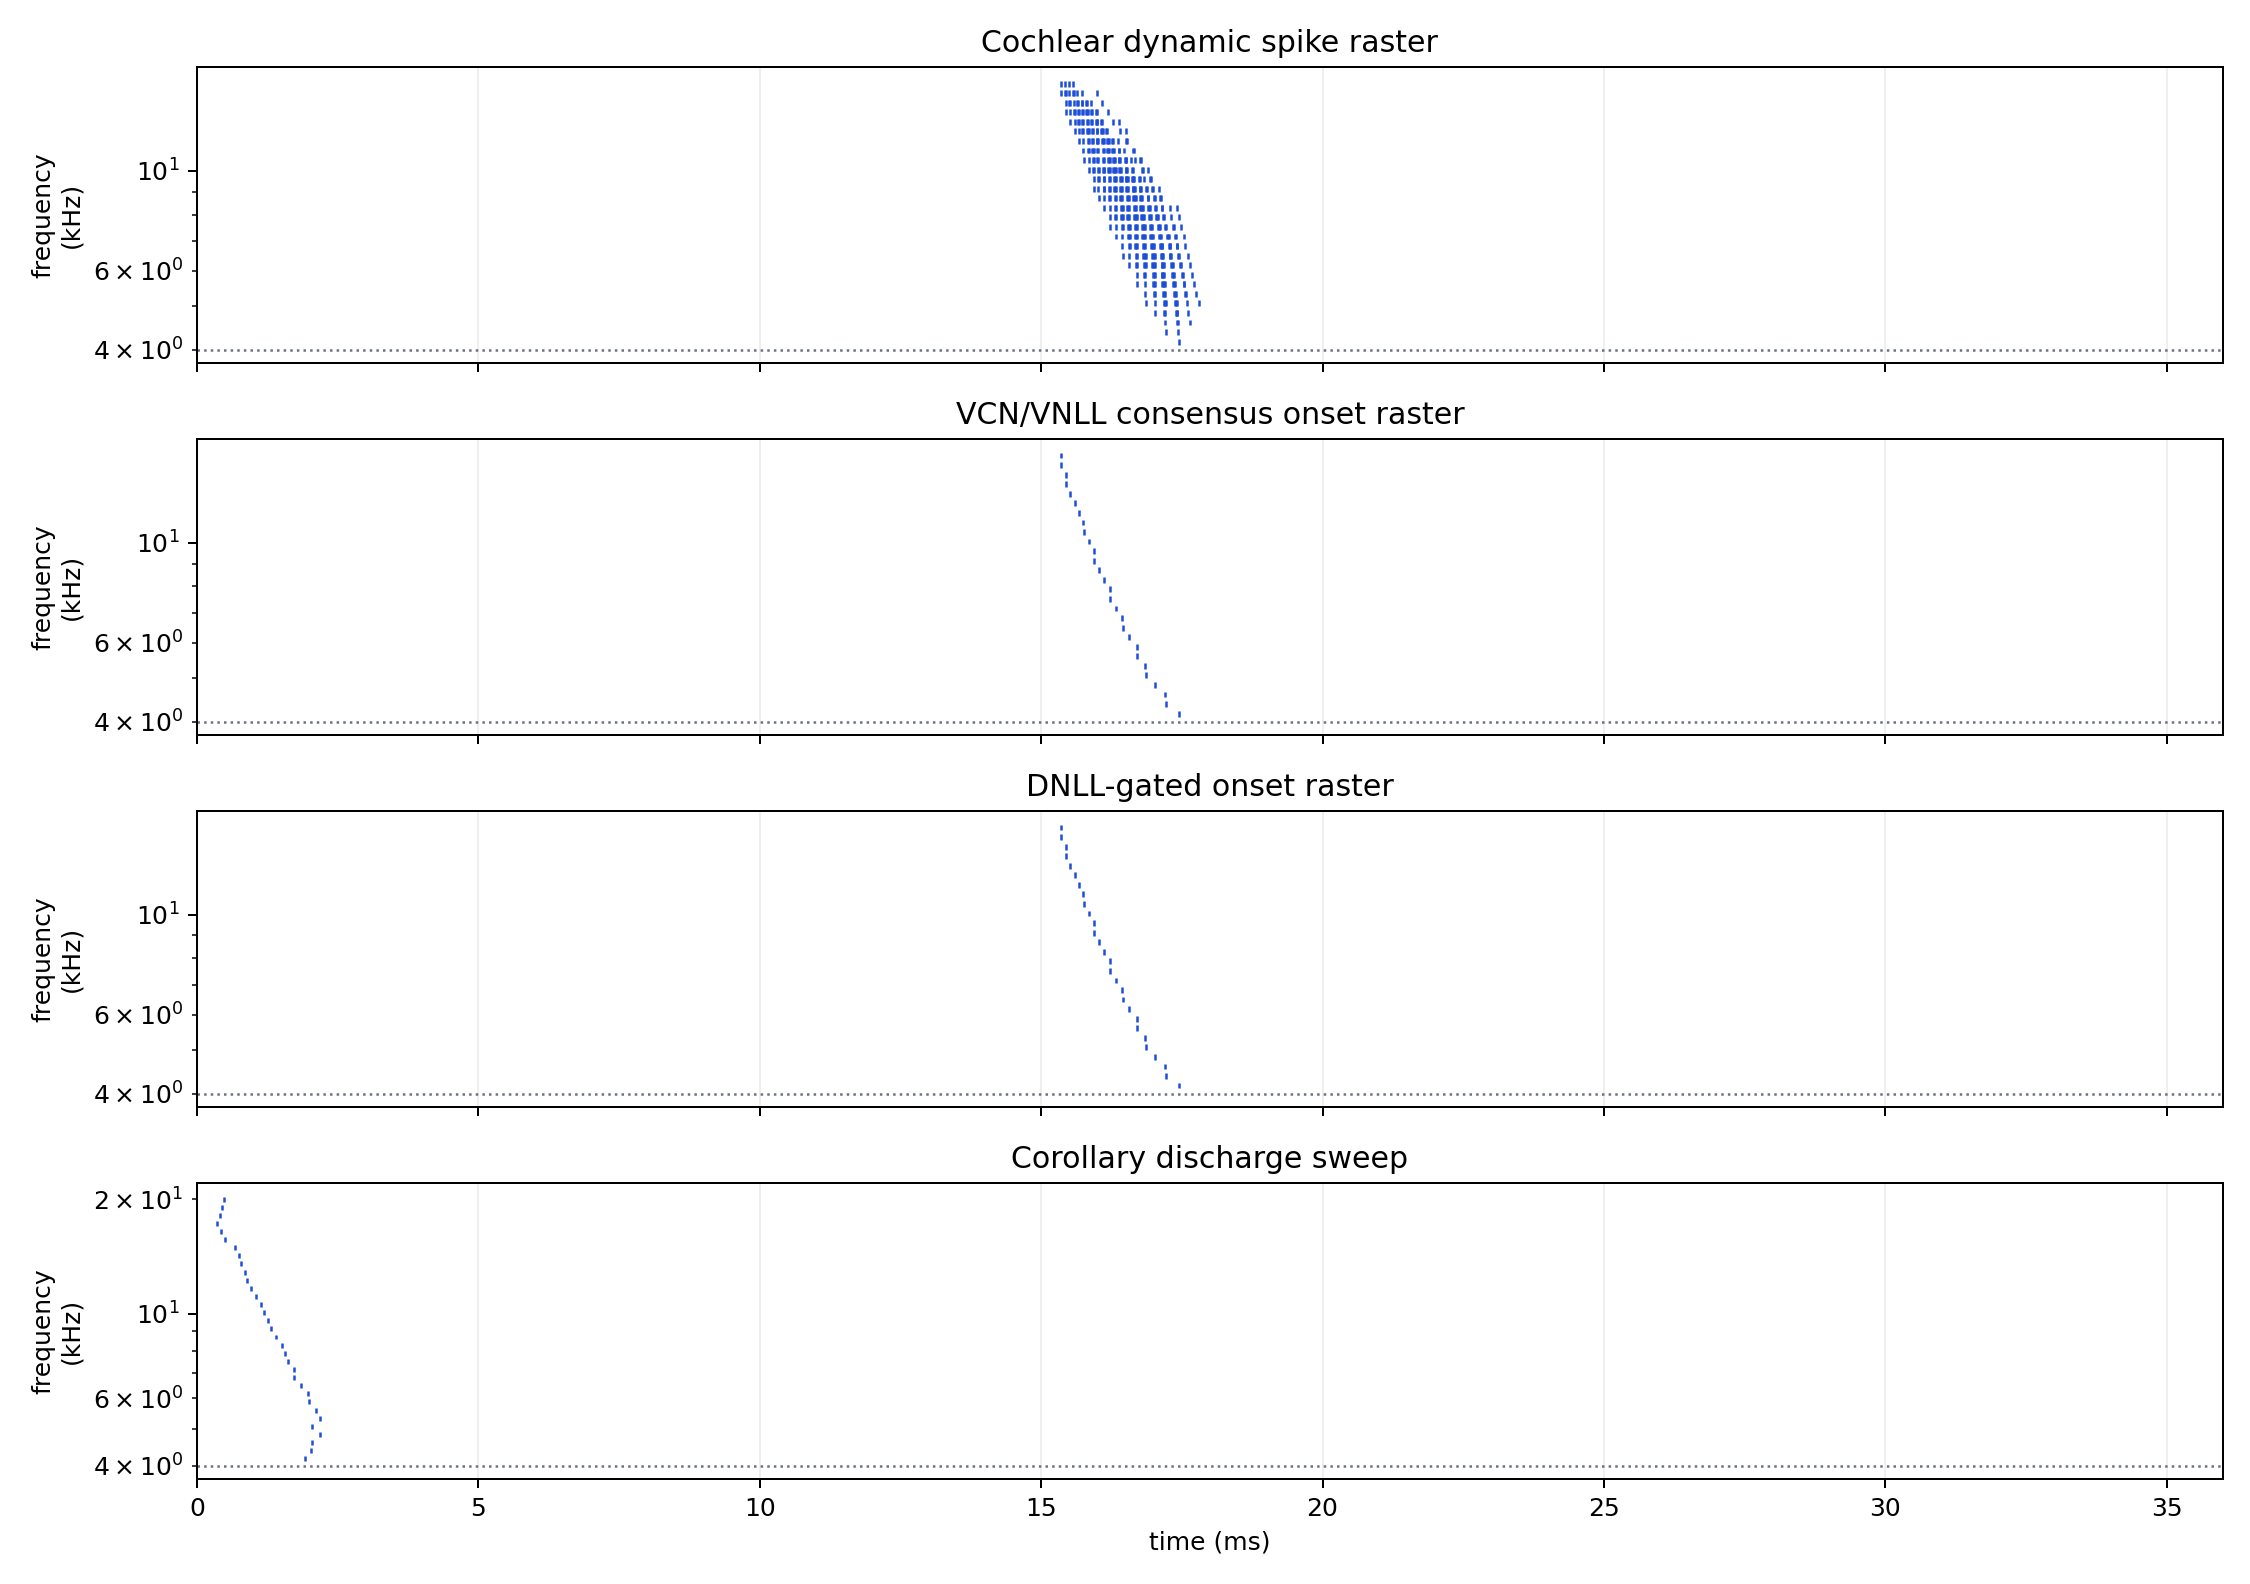
\includegraphics[width=\figwidth\linewidth]{ch4_distance_rasters.png}
  \caption{Stage-by-stage distance pathway rasters. The cochlear sweep is converted into sharpened onset activity before coincidence detection and topographic readout.}
\end{figure}

\subsection{Validation Results}

The final distance pathway was evaluated in clean and noisy tests. In the small clean 0.25--5 m test, the no-attractor centre-of-mass readout achieved 3.57 cm mean absolute error, while the reflected two-block attractor achieved 3.54 cm. In full clean three-dimensional tests up to 5 m, the reflected attractor achieved 2.66 cm mean absolute error. In full tests up to 10 m, the error rose to 34.0 cm, showing that the current tuning is strongest in the near-field operating range.

\begin{table}[H]
  \centering
  \caption{Representative distance pathway performance.}
  \begin{tabular}{llll}
    \toprule
    Test & Readout & Range & MAE\\
    \midrule
    Small clean & Centre of mass & 0.25--5 m & 0.0357 m\\
    Small clean & Reflected CANN & 0.25--5 m & 0.0354 m\\
    Small noisy & Centre of mass & 0.25--5 m & 0.0713 m\\
    Full 3D clean & Reflected CANN & up to 5 m & 0.0266 m\\
    Full 3D clean & Centre of mass & up to 10 m & 0.3404 m\\
    Full 3D, 50 dB floor & Reflected CANN & up to 5 m & 0.0266 m\\
    \bottomrule
  \end{tabular}
\end{table}

\begin{figure}[H]
  \centering
  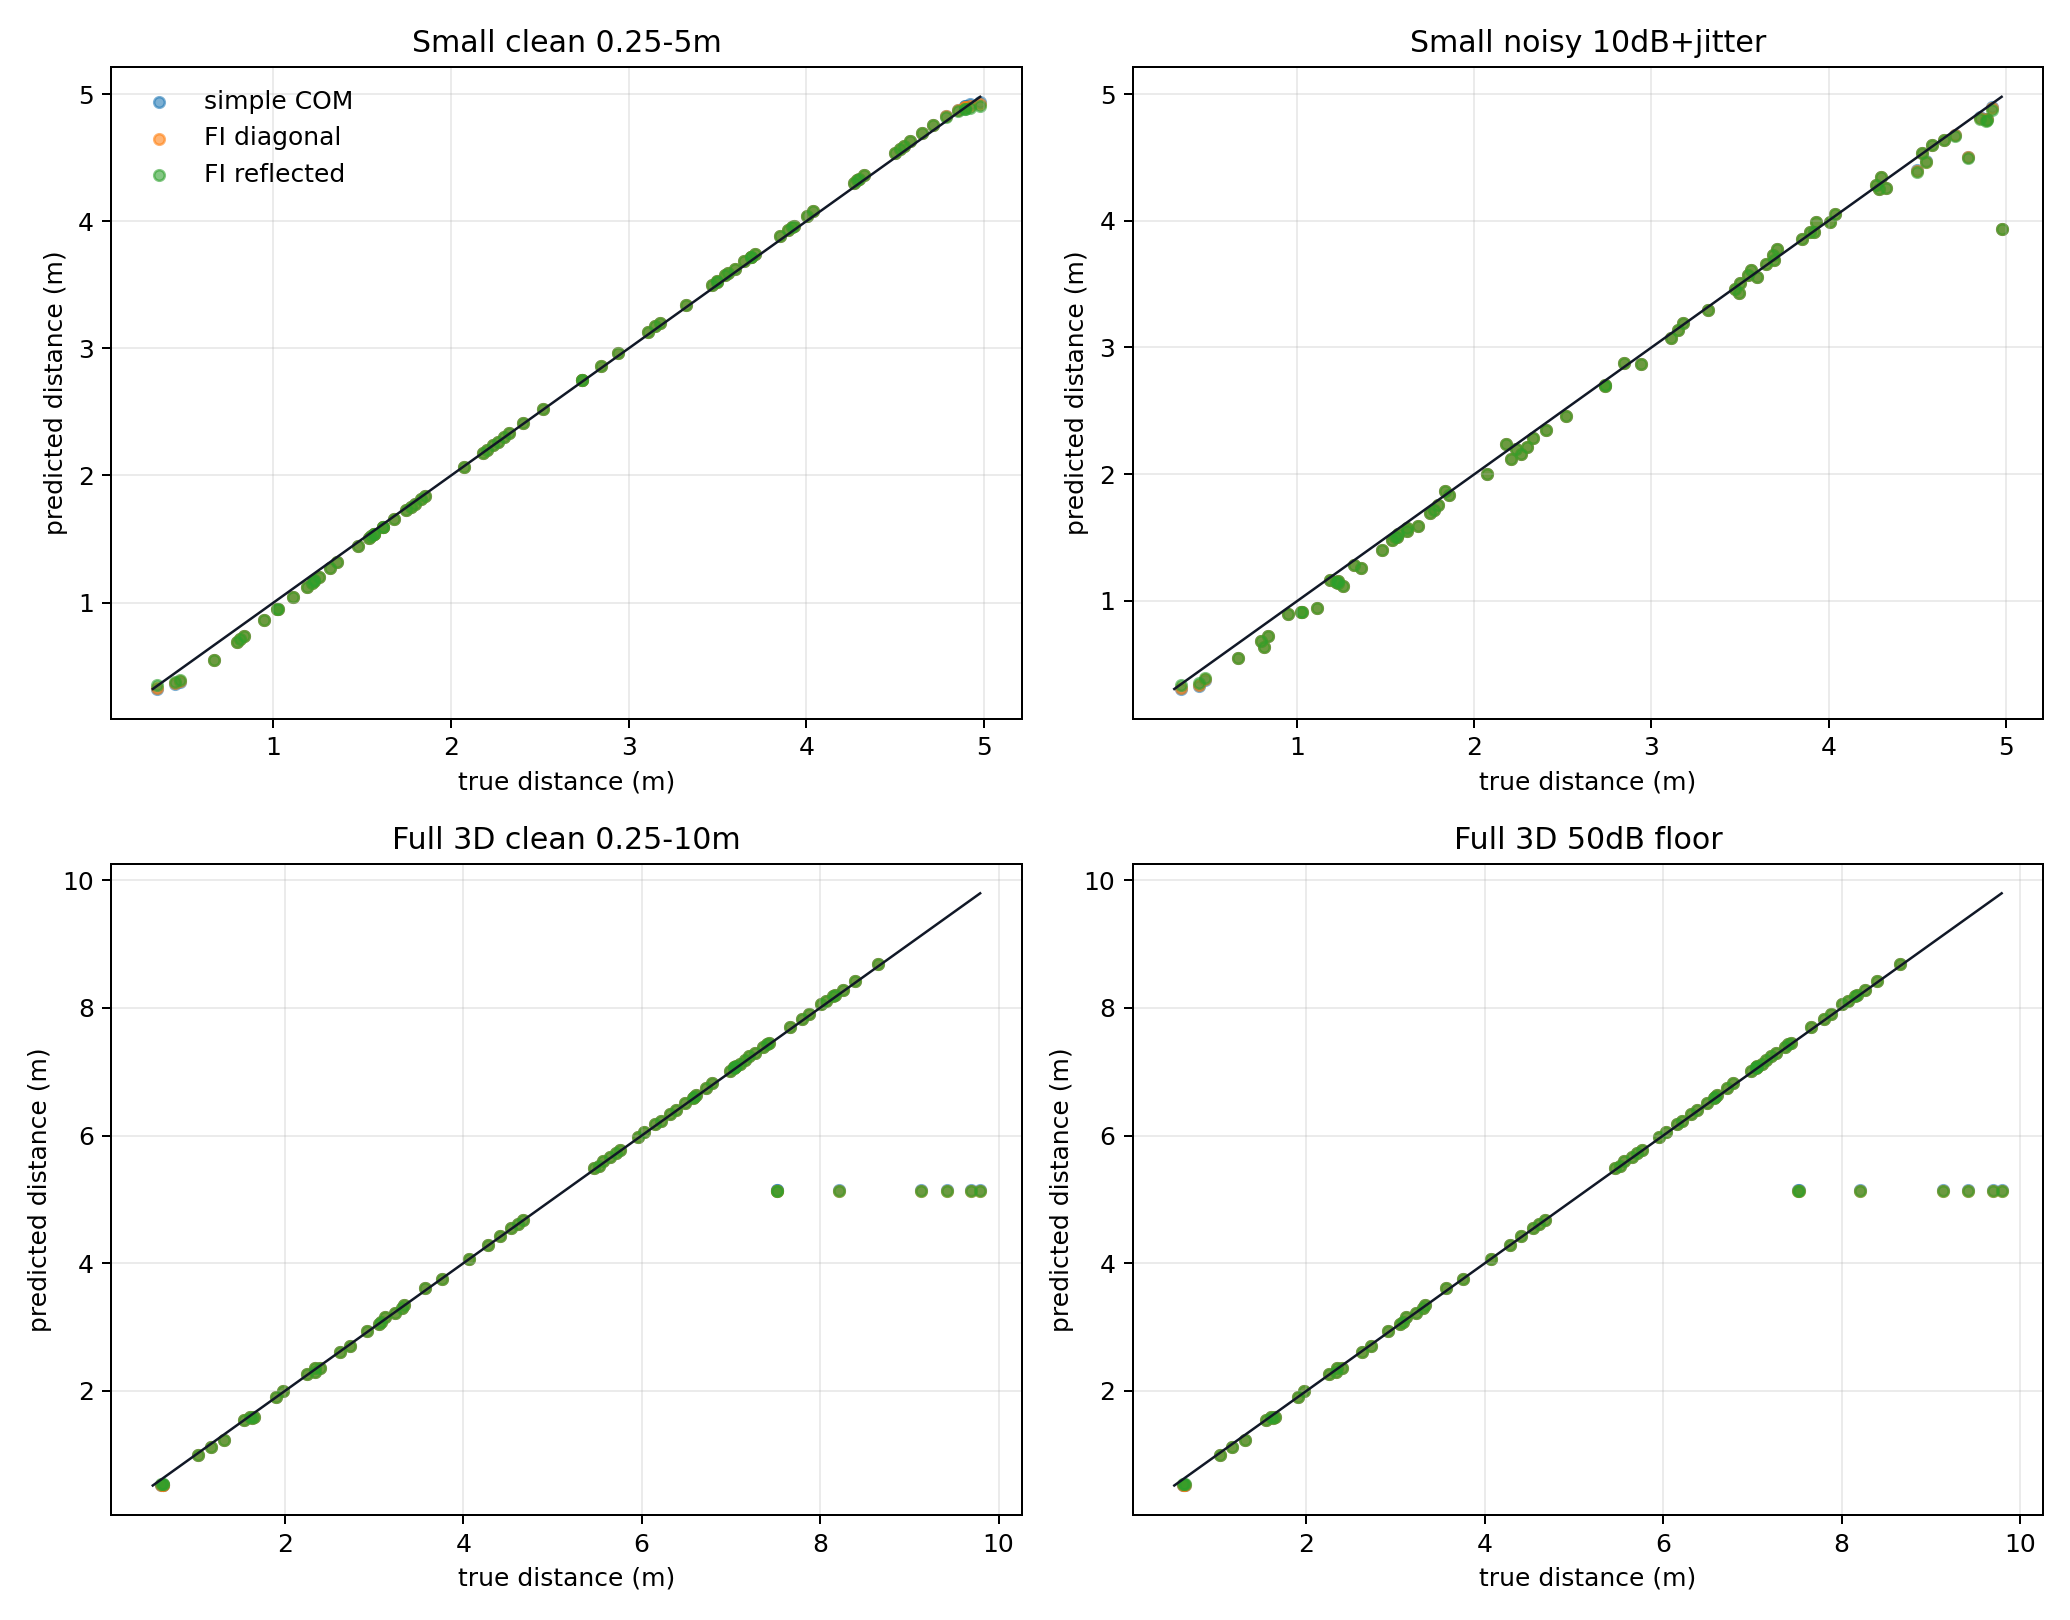
\includegraphics[width=\figwidth\linewidth]{ch4_distance_readout_scatter.png}
  \caption{Distance readout scatter for the final distance pathway. Most near-field errors are small, with larger failures appearing as the signal becomes weak or timing is corrupted.}
\end{figure}

\section{Azimuth Pathway}

\subsection{Biological Mechanism}

Azimuth estimation uses binaural information. Two main cues are available: interaural time difference (ITD), caused by different arrival times at the two ears, and interaural level difference (ILD), caused by head shadowing. The model implements both but found that the engineered ILD pathway was stronger in the tested regime.

\begin{figure}[H]
  \centering
  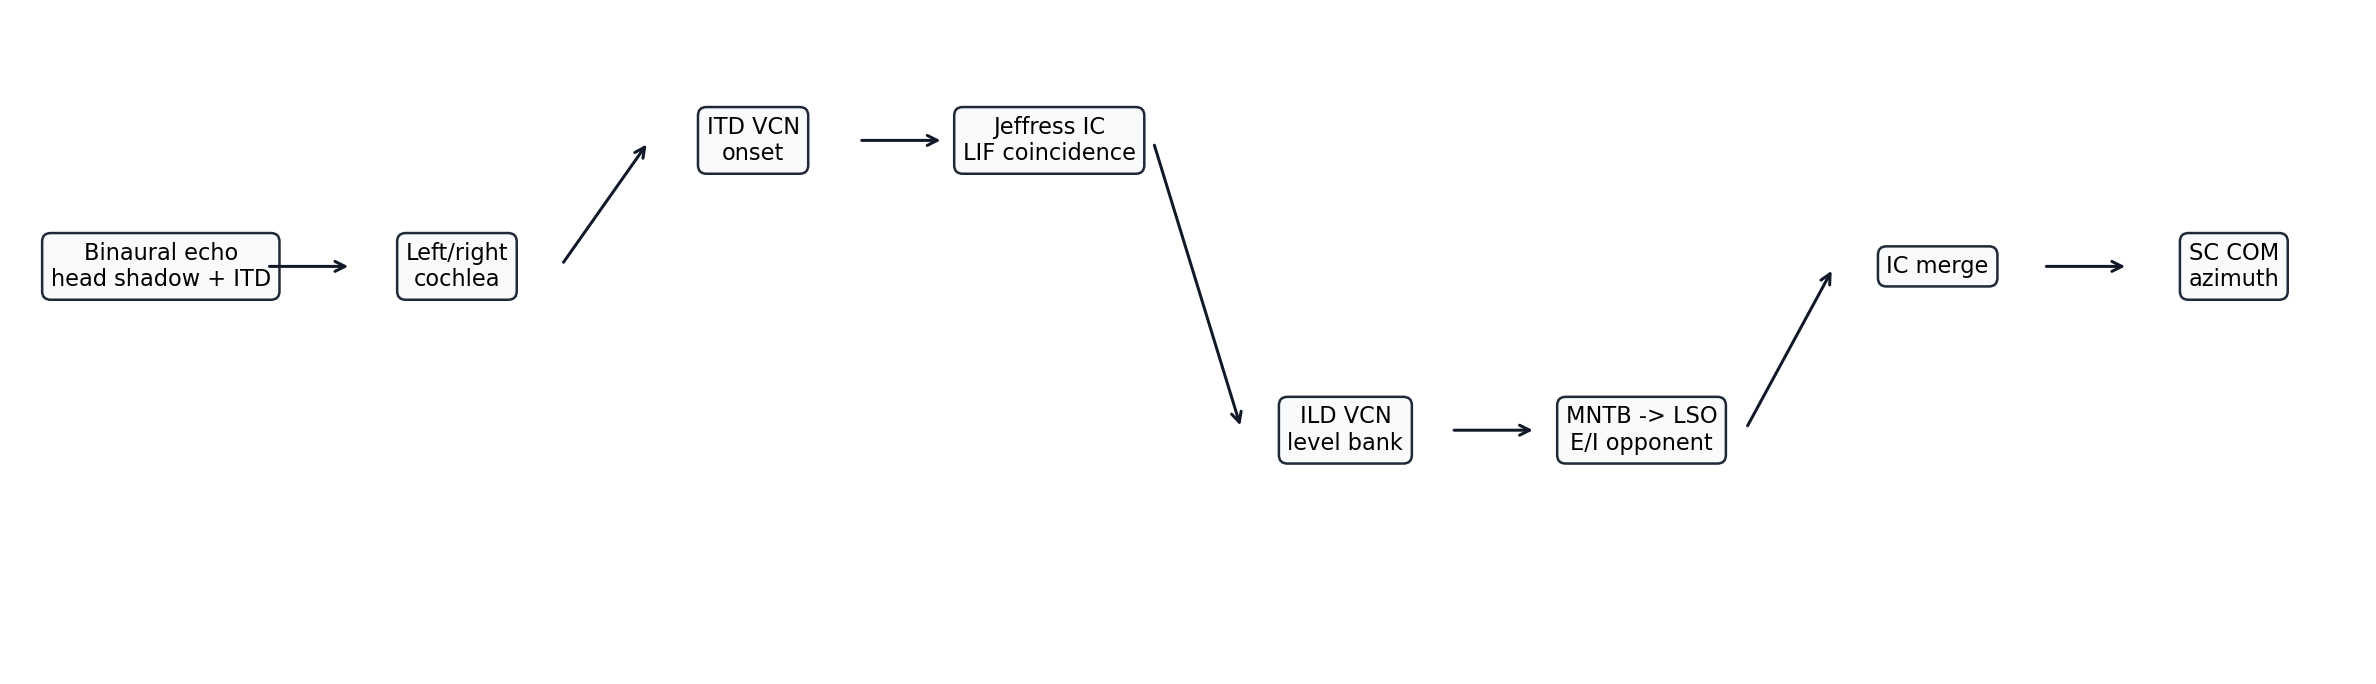
\includegraphics[width=\figwidth\linewidth]{ch4_azimuth_pipeline.png}
  \caption{Azimuth pathway stages. Binaural cochlear processing is split into ITD and ILD systems before population-code readout.}
\end{figure}

\subsection{ITD Processing}

The ITD branch uses a Jeffress-style delay-line coincidence model. If $L[t]$ and $R[t]$ are left and right onset spike trains, the score for candidate interaural delay $\delta_k$ is
\[
  J[k] = \sum_t L[t]R[t-\delta_k].
\]
This is biologically interpretable and works well when timing is reliable. However, at the 64 kHz sample rate and with the current ear spacing, the available ITD range is small and quantisation limits performance.

\subsection{ILD Processing}

The ILD branch compares binaural spike counts. A simplified level ratio is
\[
  \ell = \log\frac{R+\epsilon}{L+\epsilon}.
\]
Because head-shadow gain is saturating with azimuth, the raw ILD-to-angle curve is sigmoid-like. The most successful correction used an inverse-sigmoid warp,
\[
  \hat{\phi} = a \operatorname{arctanh}(b\ell),
\]
with clipping for numerical stability. This converts the compressed ILD cue into a more linear azimuth estimate over the tuned range.

\begin{figure}[H]
  \centering
  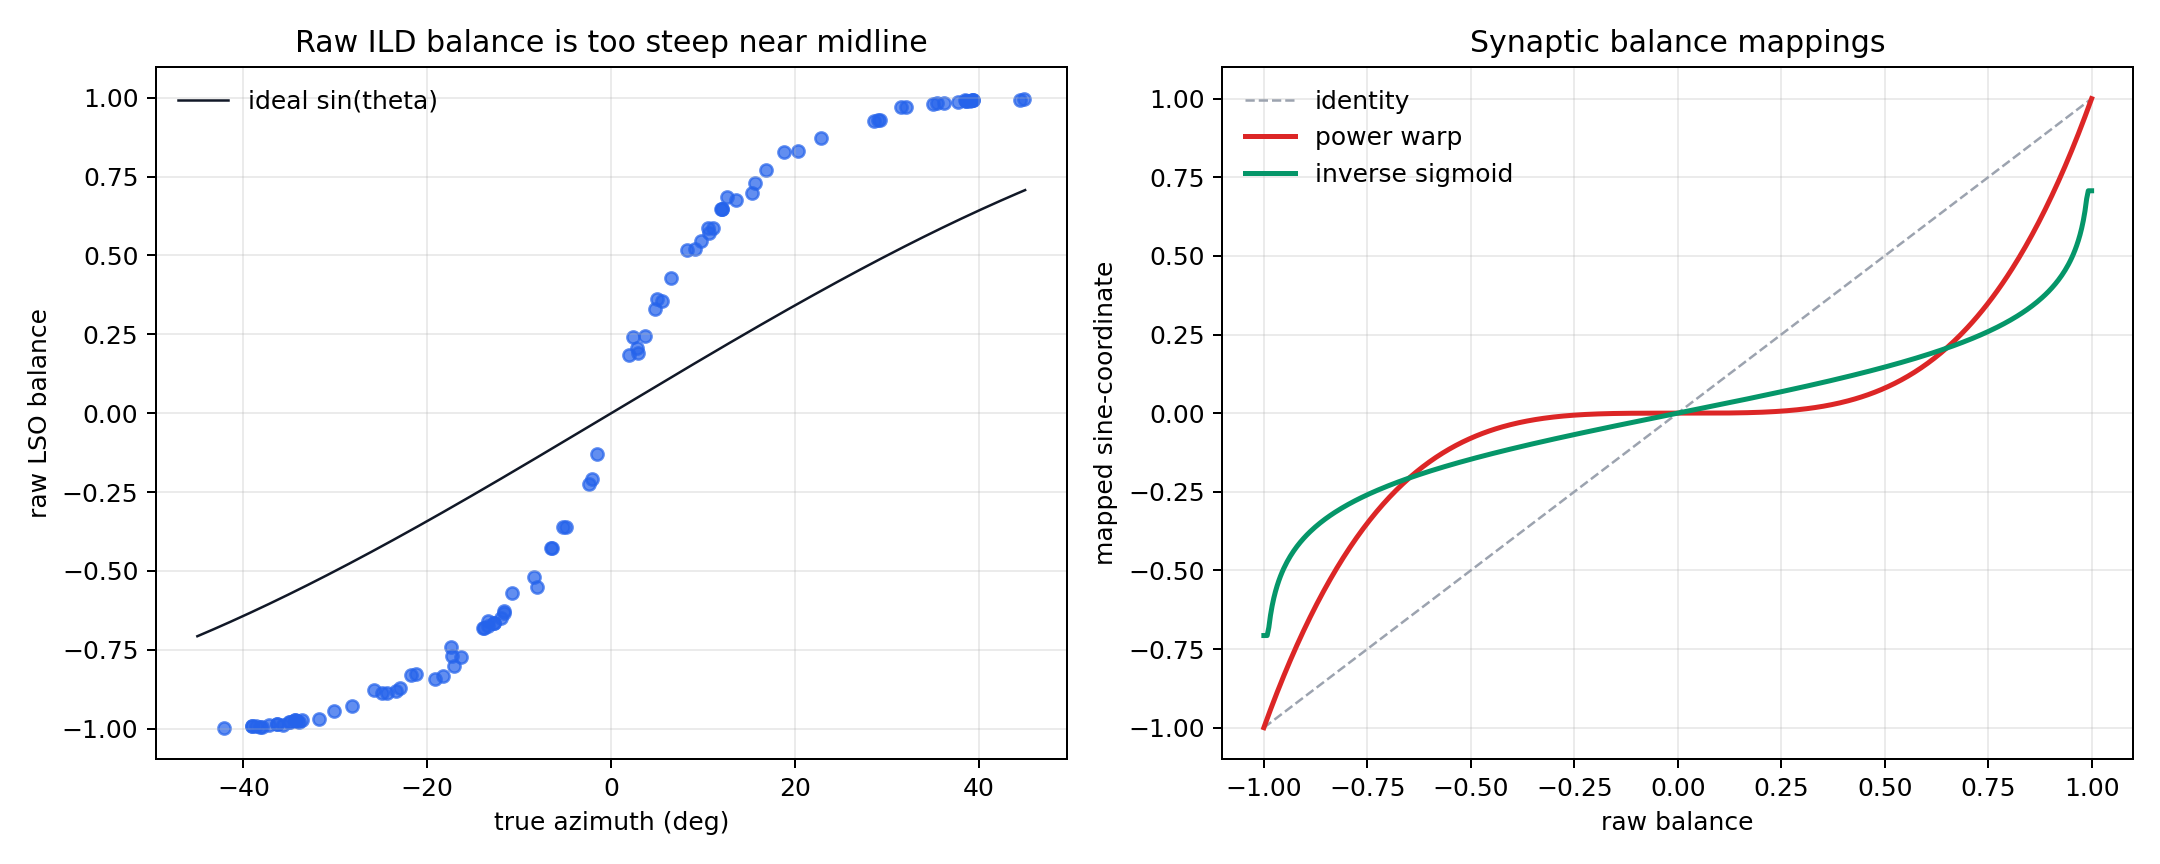
\includegraphics[width=\figwidth\linewidth]{ch4_azimuth_warped_ild.png}
  \caption{Inverse-sigmoid ILD warping. The warp corrects the saturating ILD response and substantially improves isolated azimuth accuracy.}
\end{figure}

\subsection{Validation Results}

In isolated $\pm45^\circ$ tests, the inverse-sigmoid ILD system achieved approximately $0.98^\circ$ mean absolute error, outperforming both the raw ILD and ITD branches. In full three-dimensional tests, the error increased to approximately $9.7^\circ$ over $\pm45^\circ$ and approximately $21^\circ$ over $\pm90^\circ$. This is expected because a pure ILD model is confounded by distance, elevation-dependent spectral filtering, and target-side geometry.

\begin{table}[H]
  \centering
  \caption{Representative azimuth pathway performance.}
  \begin{tabular}{lll}
    \toprule
    Test & Model & Azimuth MAE\\
    \midrule
    Isolated $\pm45^\circ$ & ITD & $1.89^\circ$\\
    Isolated $\pm45^\circ$ & Raw ILD & $11.80^\circ$\\
    Isolated $\pm45^\circ$ & Inverse-sigmoid ILD & $0.98^\circ$\\
    Isolated stress & Inverse-sigmoid ILD & $7.73^\circ$\\
    Full 3D $\pm45^\circ$, up to 5 m & ILD CANN & $9.63^\circ$\\
    Full 3D $\pm90^\circ$ & ILD CANN & $20.84^\circ$\\
    \bottomrule
  \end{tabular}
\end{table}

\begin{figure}[H]
  \centering
  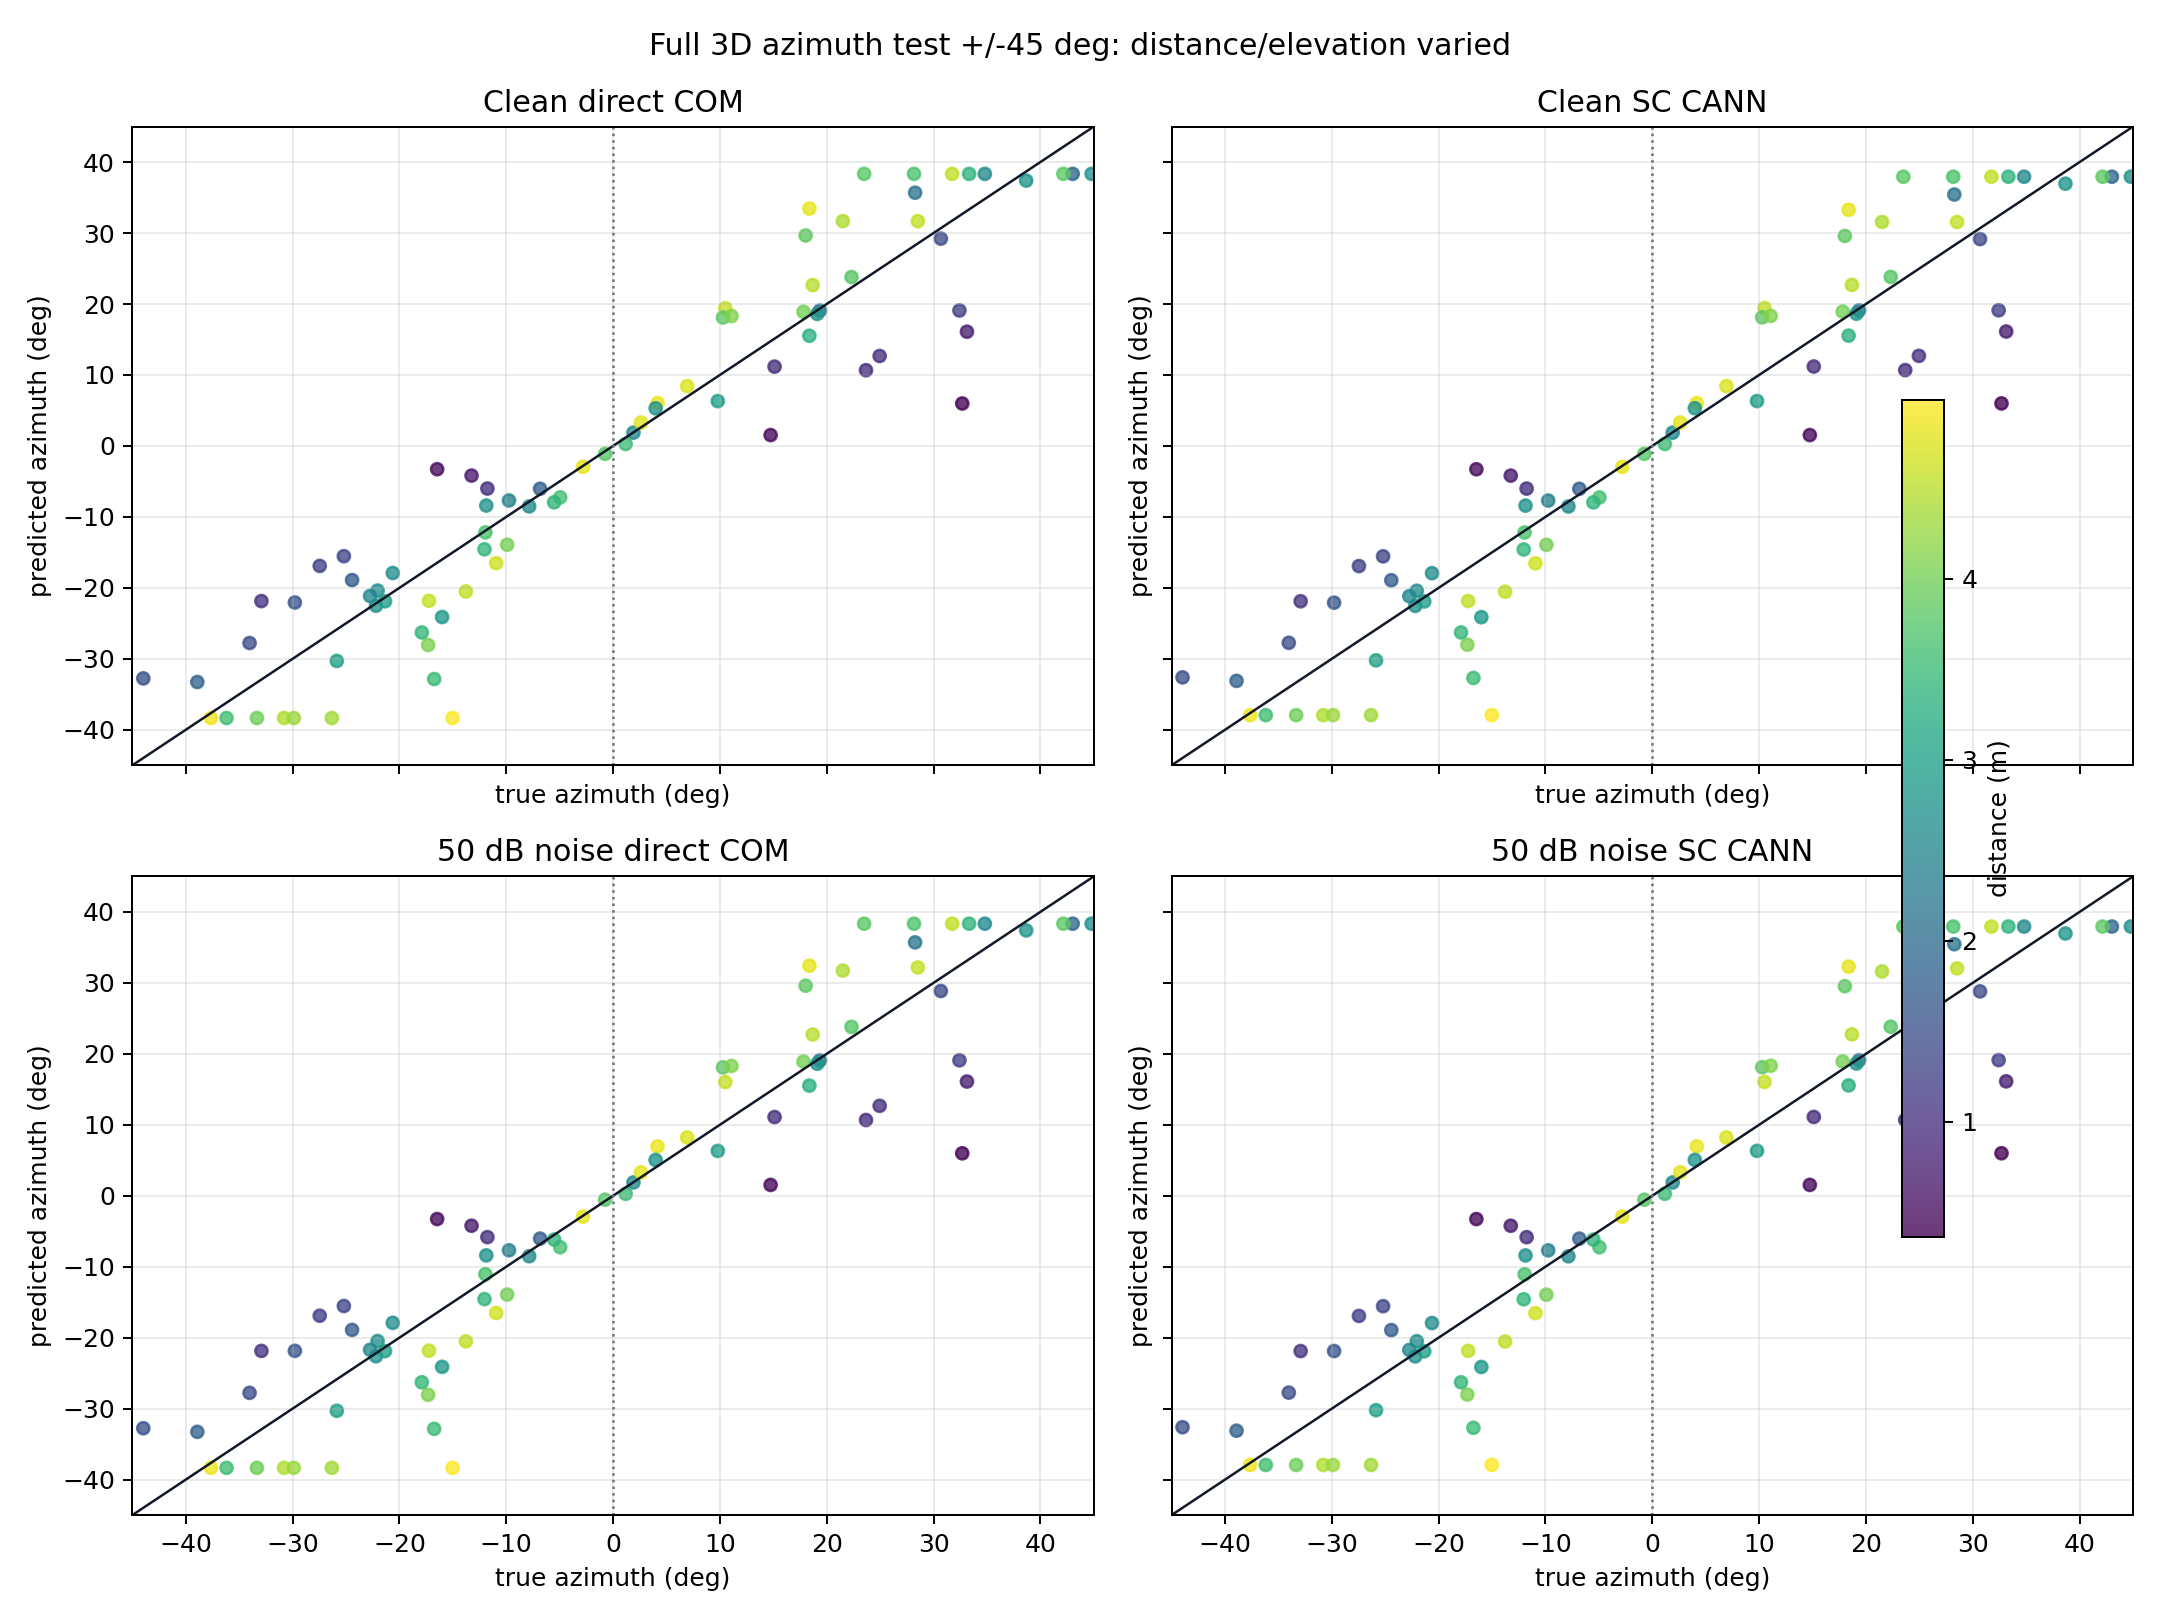
\includegraphics[width=\figwidth\linewidth]{ch4_azimuth_full3d_pm45.png}
  \caption{Full three-dimensional azimuth test over $\pm45^\circ$. The trend remains visible, but full-scene confounds reduce accuracy compared with isolated azimuth sweeps.}
\end{figure}

\section{Elevation Pathway}

\subsection{Biological Mechanism}

Elevation is mainly a spectral cue. In mammals, pinna and outer-ear filtering create elevation-dependent spectral notches. The dorsal cochlear nucleus is often associated with spectral-shape processing. The model therefore uses a monaural DCN-style template system: cochlear channels project to elevation-tuned neurons with excitatory and inhibitory weights derived from the expected spectral transfer function.

\subsection{Comb-Filter Spectral Cue}

The final elevation experiments used a comb-filter notch rather than the earlier broad Gaussian notch. The filtered signal is
\[
  y(t) = x(t) + a x(t-\tau),
\]
with frequency response
\[
  H(f) = 1 + a e^{-j2\pi f \tau},
\]
\[
  |H(f)|^2 = 1 + a^2 + 2a\cos(2\pi f \tau).
\]
Changing $\tau$ changes the notch frequencies. The elevation model maps each candidate elevation angle to a candidate transfer function and uses this as a synaptic template.

\begin{figure}[H]
  \centering
  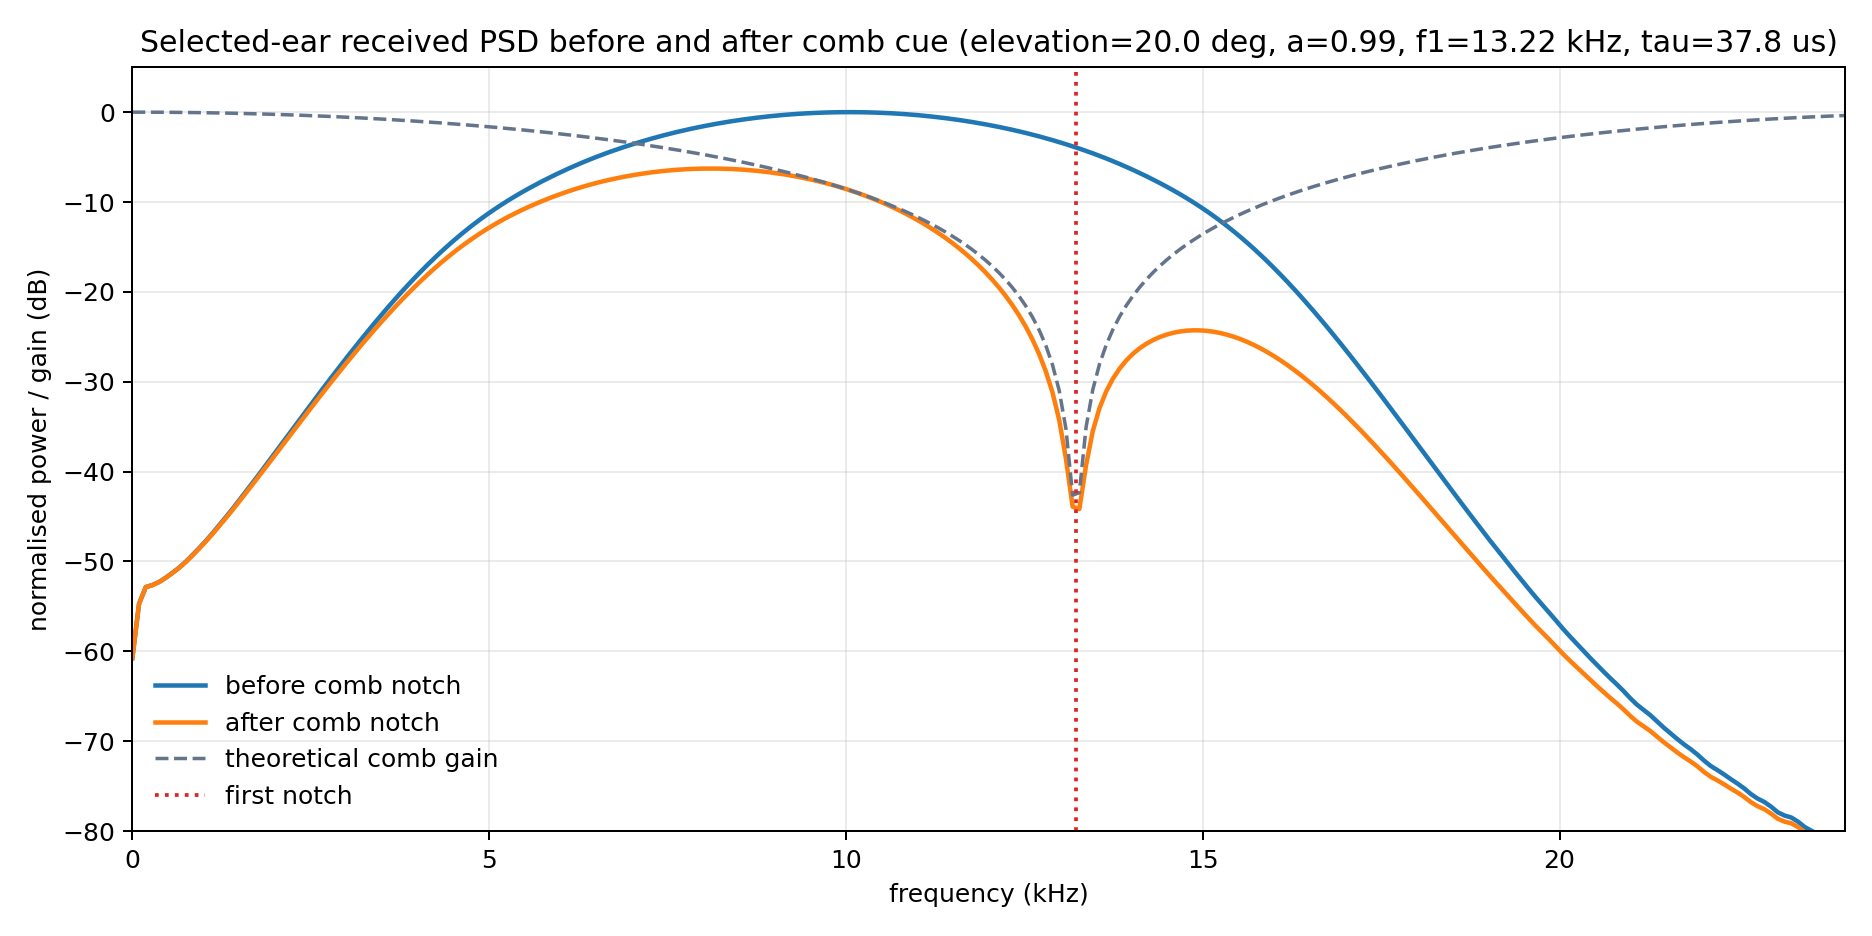
\includegraphics[width=\figwidth\linewidth]{ch4_elevation_deep_psd.png}
  \caption{Power spectral density before and after the deep comb-filter notch. The notch must be visible in the received spectrum before a downstream DCN template can detect it.}
\end{figure}

\subsection{DCN Template Model}

The most successful model used signal-weighted full-transfer templates. If $P_0(f)$ is the baseline signal power and $H_{\theta}(f)$ is the elevation-dependent transfer function, the expected template for elevation $\theta$ is based on
\[
  T_{\theta}(f) \propto P_0(f)|H_{\theta}(f)|^2.
\]
This matters because the emitted chirp and cochlea do not create a flat frequency response. A template based only on the notch transfer function can place excessive weight on frequencies where the actual signal has little power.

\begin{figure}[H]
  \centering
  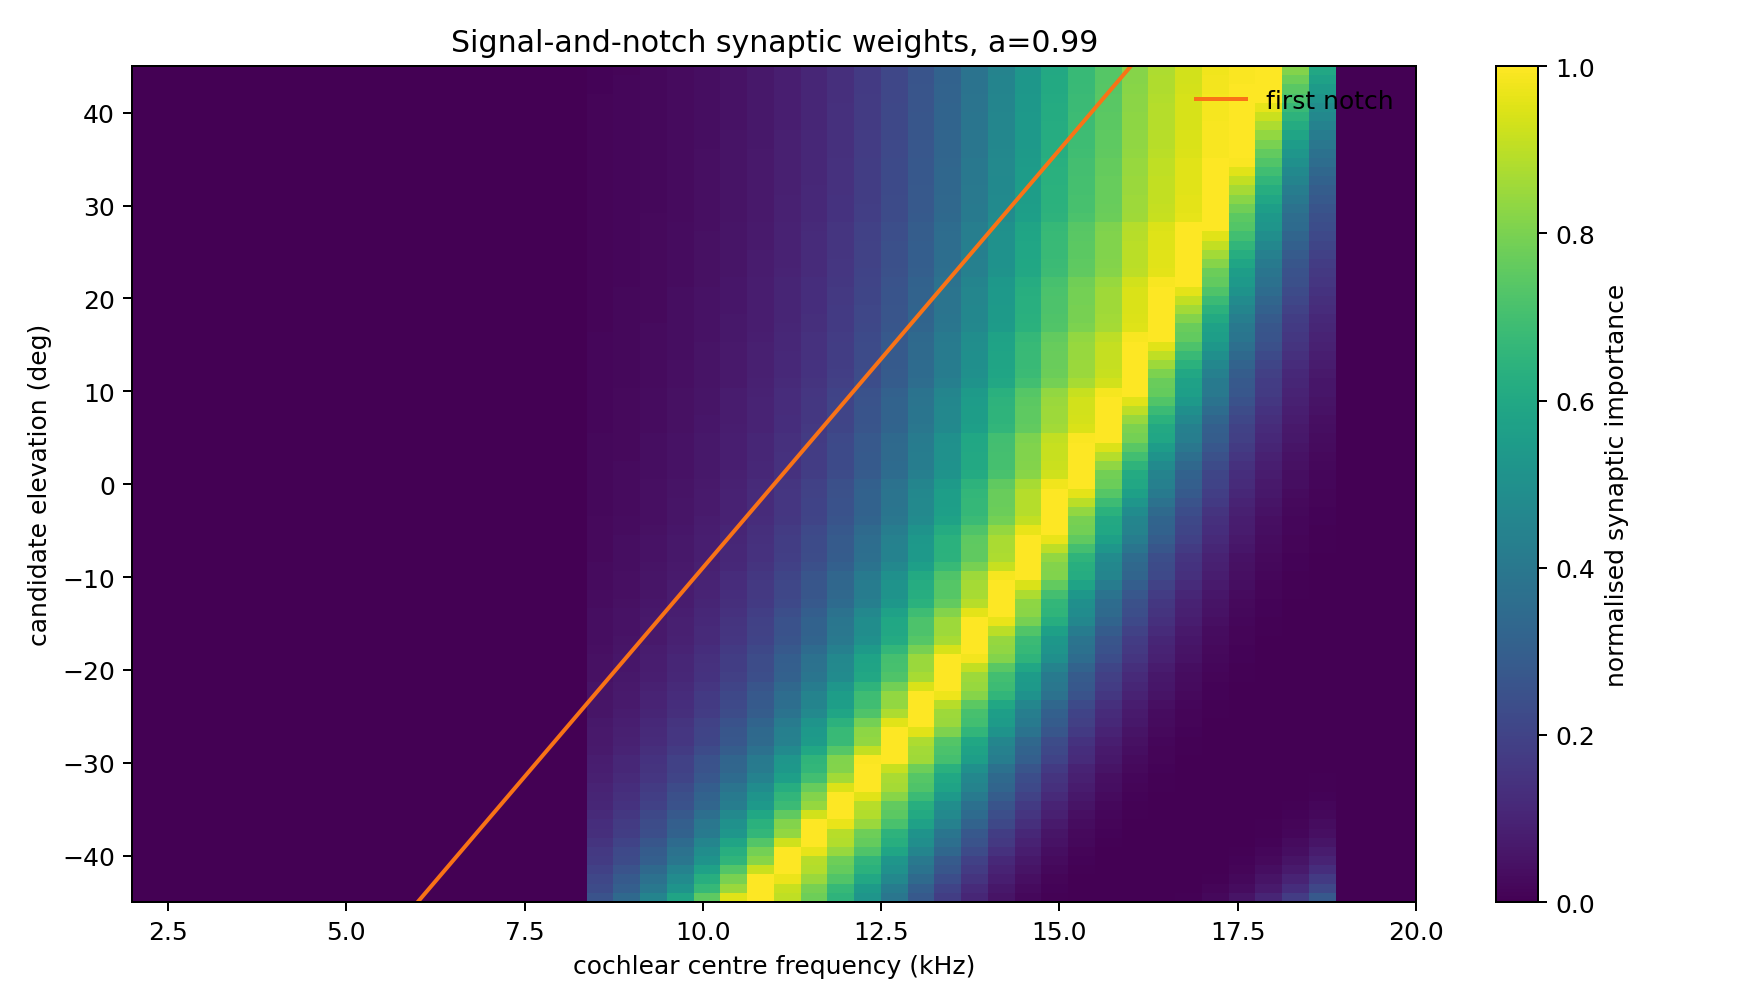
\includegraphics[width=\figwidth\linewidth]{ch4_elevation_synaptic_weights.png}
  \caption{Elevation pathway synaptic weights. The DCN bank maps cochlear frequency channels to elevation-tuned neurons using a signal-weighted spectral template.}
\end{figure}

\subsection{Validation Results}

The best isolated elevation model was the deep-comb signal-weighted full-transfer DCN centre-of-mass model, achieving approximately $2.82^\circ$ mean absolute error. In clean full three-dimensional tests up to 5 m, the same design achieved approximately $3.03^\circ$ mean absolute error. Attempts to add lateral inhibition and dynamic wideband inhibition did not improve the clean full-three-dimensional result in the tested grid, most likely because the already narrow comb template was over-sharpened.

\begin{table}[H]
  \centering
  \caption{Representative elevation pathway performance.}
  \begin{tabular}{ll}
    \toprule
    Model & Elevation MAE\\
    \midrule
    Local-dip COM & $16.91^\circ$\\
    Explicit E/I profile COM & $7.10^\circ$\\
    Signal-weighted full-transfer COM & $3.14^\circ$\\
    Deep-comb signal-weighted full-transfer COM & $2.82^\circ$\\
    Full 3D clean, up to 5 m & $3.03^\circ$\\
    \bottomrule
  \end{tabular}
\end{table}

\begin{figure}[H]
  \centering
  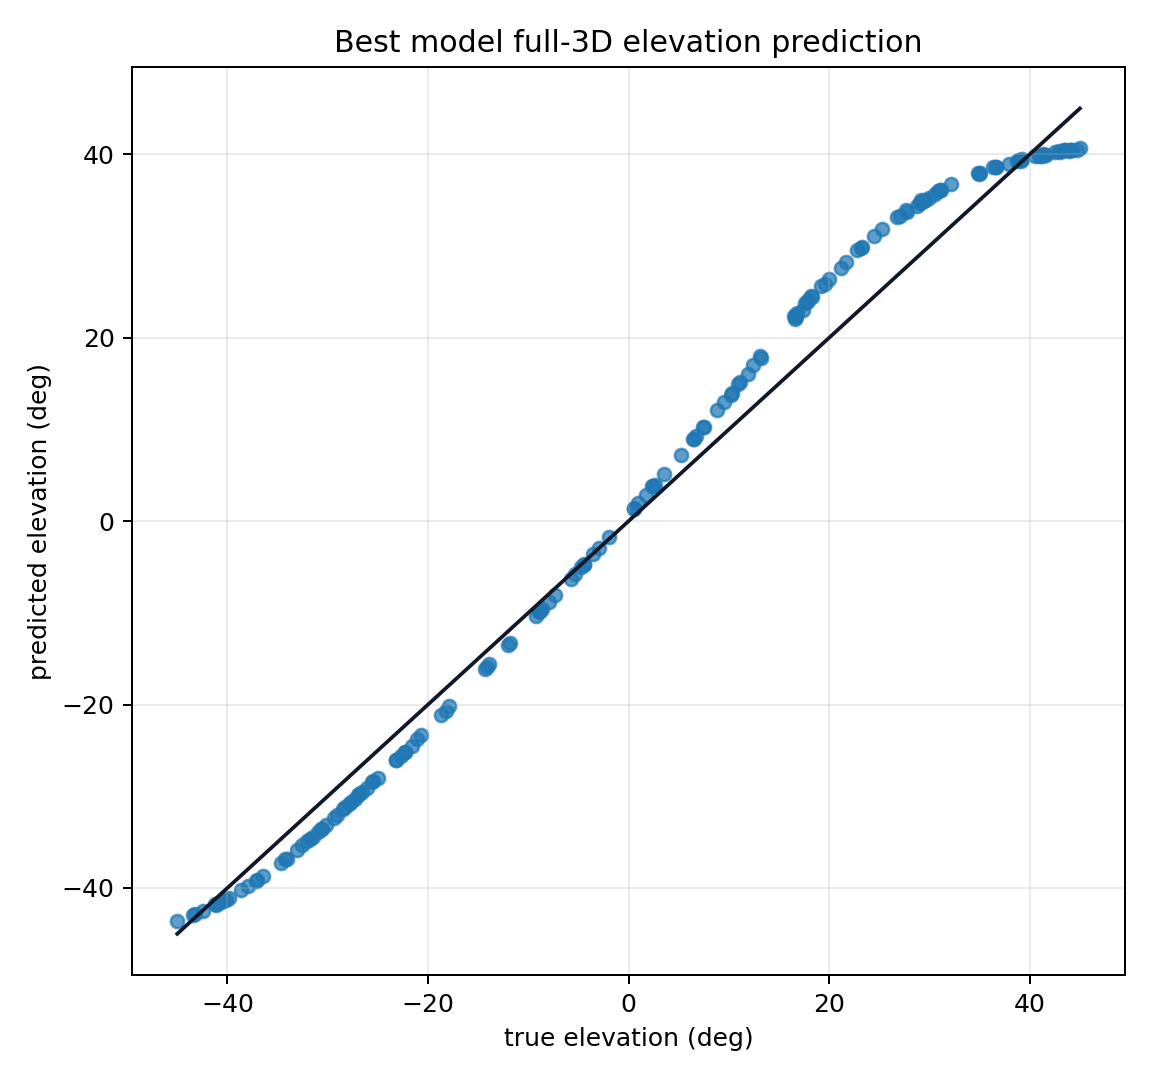
\includegraphics[width=\figwidth\linewidth]{ch4_elevation_full3d_scatter.png}
  \caption{Full three-dimensional elevation scatter. The monaural spectral pathway remains useful in the full scene, unlike the azimuth ILD cue which is more strongly distance-confounded.}
\end{figure}

\chapter{Cortical Integration and Continuous Attractor Dynamics}

\section{Population Codes}

Each pathway ultimately produces a population code: a vector of activity over candidate distances, azimuths, or elevations. A simple centre-of-mass decoder treats this activity as a posterior-like distribution. However, biological spatial maps often contain recurrent dynamics, and a continuous attractor neural network provides a principled way to smooth and stabilise these population codes.

\section{Line Attractor Model}

The line attractor is modelled as
\[
  \tau \frac{d\mathbf{r}}{dt} = -\mathbf{r} + \left[W\mathbf{r} + B\mathbf{u}\right]_+,
\]
where $\mathbf{r}$ is the attractor activity, $W$ is recurrent connectivity, $B$ maps input population activity into the attractor, and $\mathbf{u}$ is the pathway input. For a ring attractor, $W$ can be circulant. For a finite line, translation invariance breaks at the boundaries, so the project tested Toeplitz, reflected, and compensated structures.

\begin{figure}[H]
  \centering
  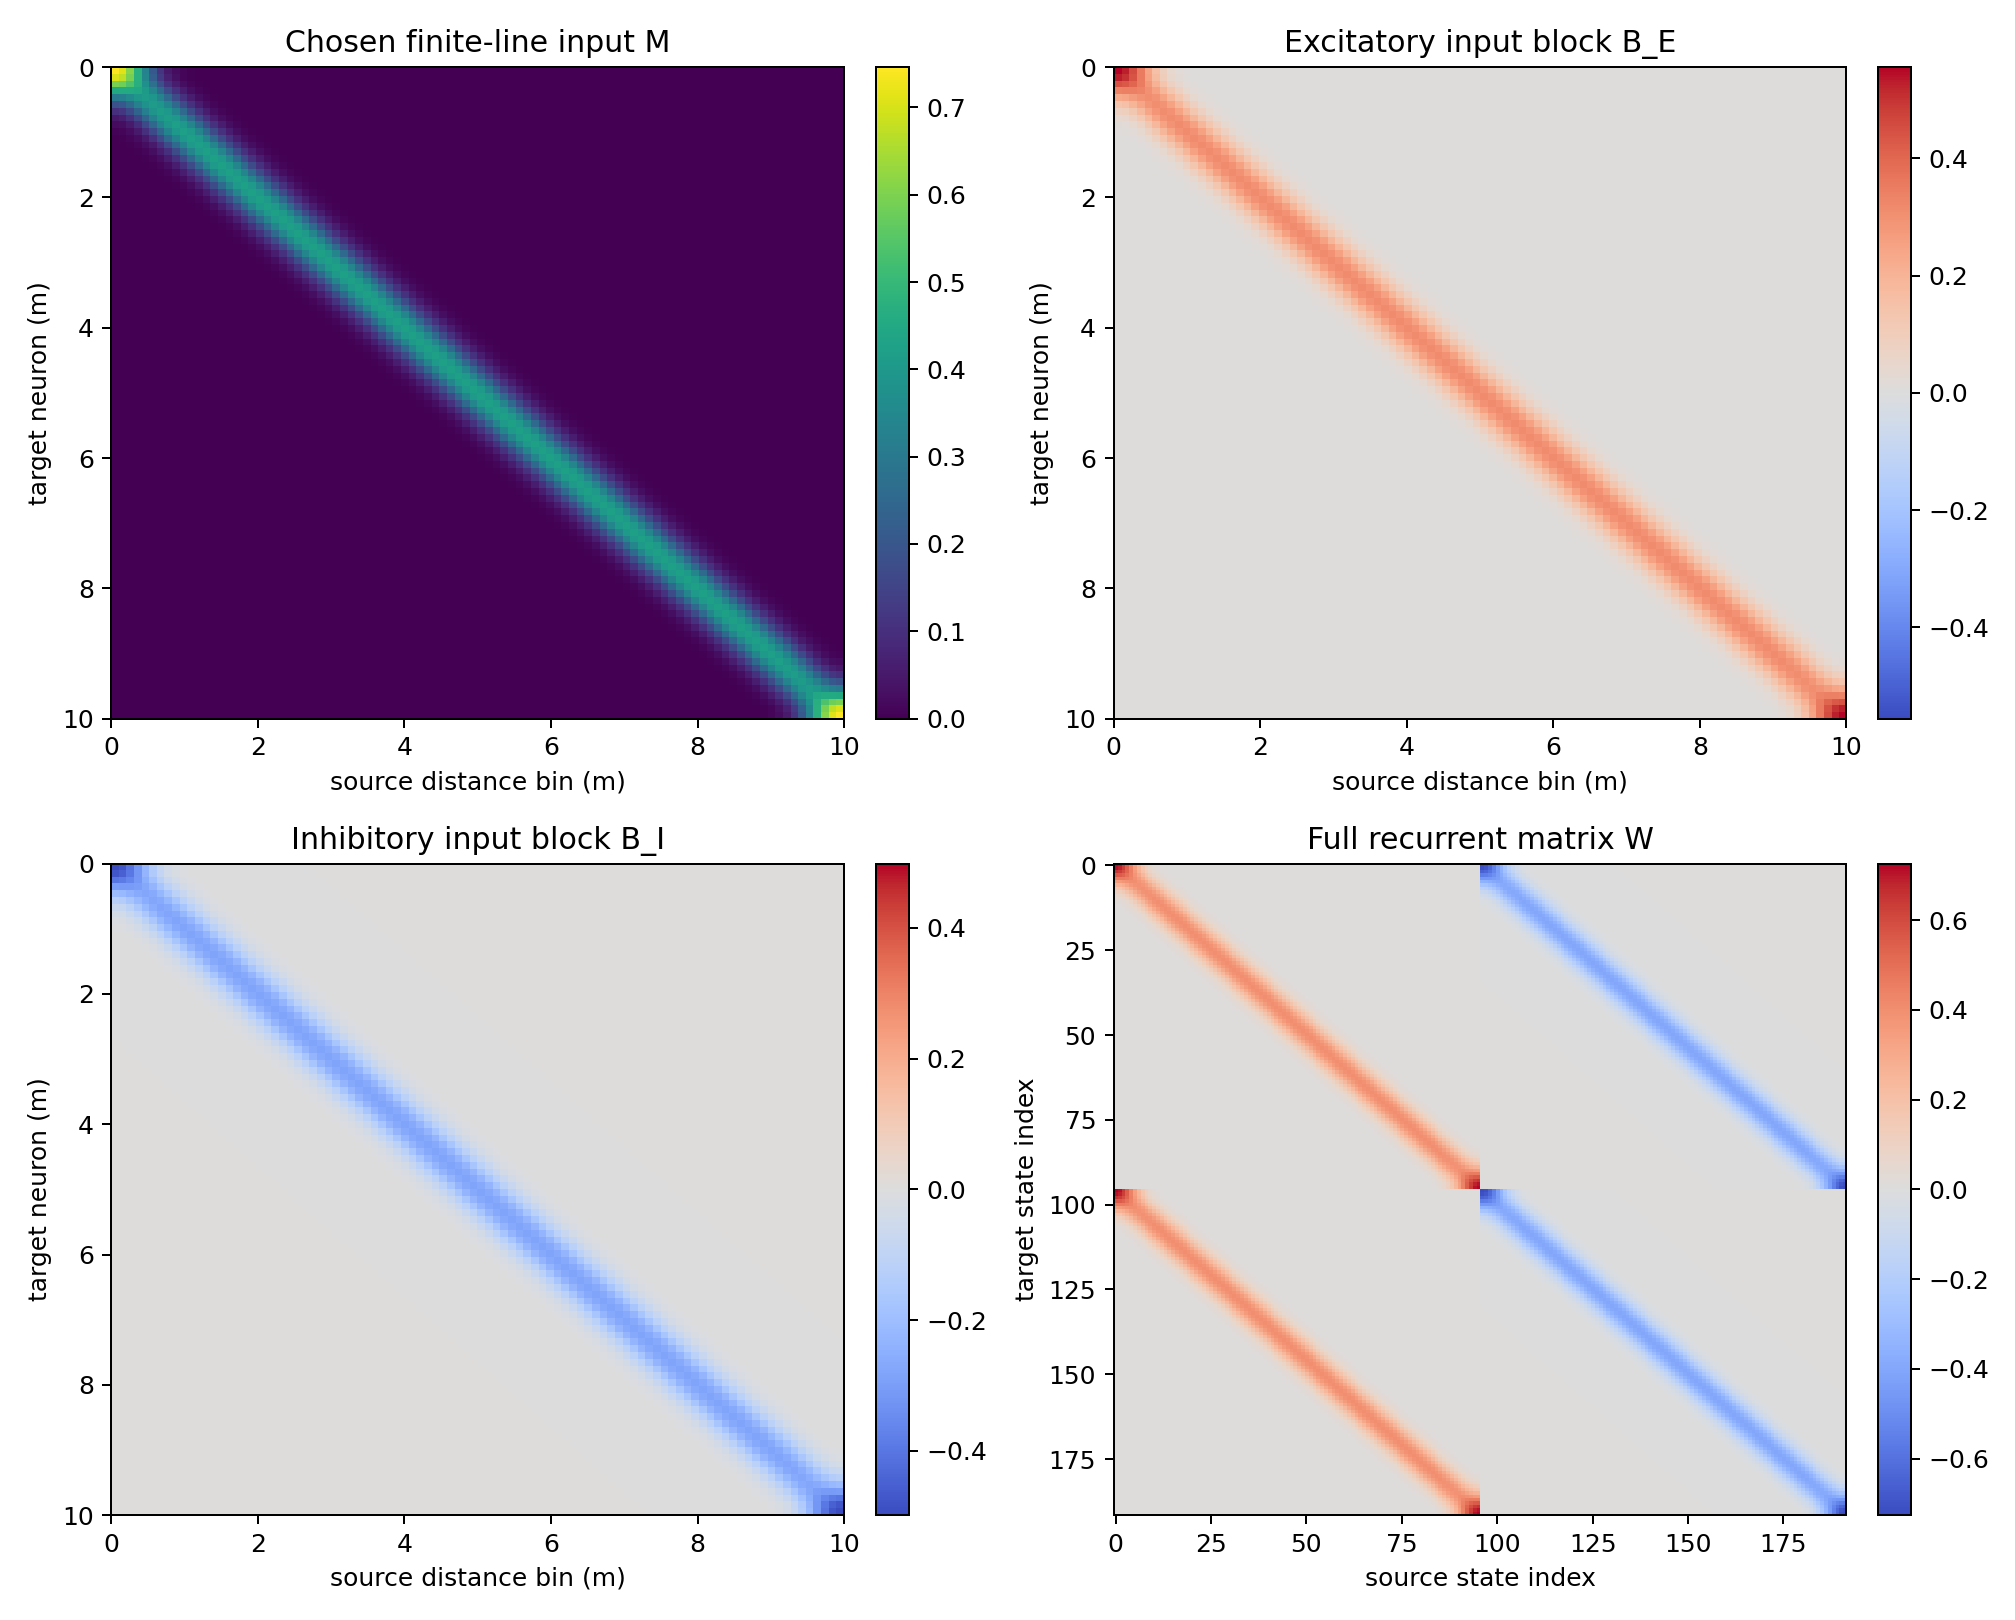
\includegraphics[width=\figwidth\linewidth]{ch5_cann_chosen_matrices.png}
  \caption{Chosen finite-line CANN matrices. The recurrence imposes local excitation and longer-range balancing, while the input matrix maps pathway activity into the line attractor.}
\end{figure}

\section{Fisher Information Motivation}

Fisher information measures how sensitively a population response changes with the encoded variable. For response mean $\boldsymbol{\mu}(x)$ and covariance $\Sigma$, the scalar Fisher information is
\[
  \mathcal{I}(x) =
  \left(\frac{\partial \boldsymbol{\mu}}{\partial x}\right)^T
  \Sigma^{-1}
  \left(\frac{\partial \boldsymbol{\mu}}{\partial x}\right).
\]
Maximising Fisher information is useful because, under regularity assumptions, the Cramer-Rao bound gives
\[
  \mathrm{Var}(\hat{x}) \geq \frac{1}{\mathcal{I}(x)}.
\]
This does not guarantee best performance in every nonlinear system, but it gives a principled criterion for selecting input weights and population widths without purely ad hoc tuning.

\section{Energy Landscape}

A CANN can be interpreted as a dynamical system whose stable states form a low-energy manifold. For a line attractor, the desired energy landscape is a trough along the represented variable. Activity should collapse toward the trough in directions orthogonal to the line, while remaining movable along the line when the input indicates a different position.

\begin{figure}[H]
  \centering
  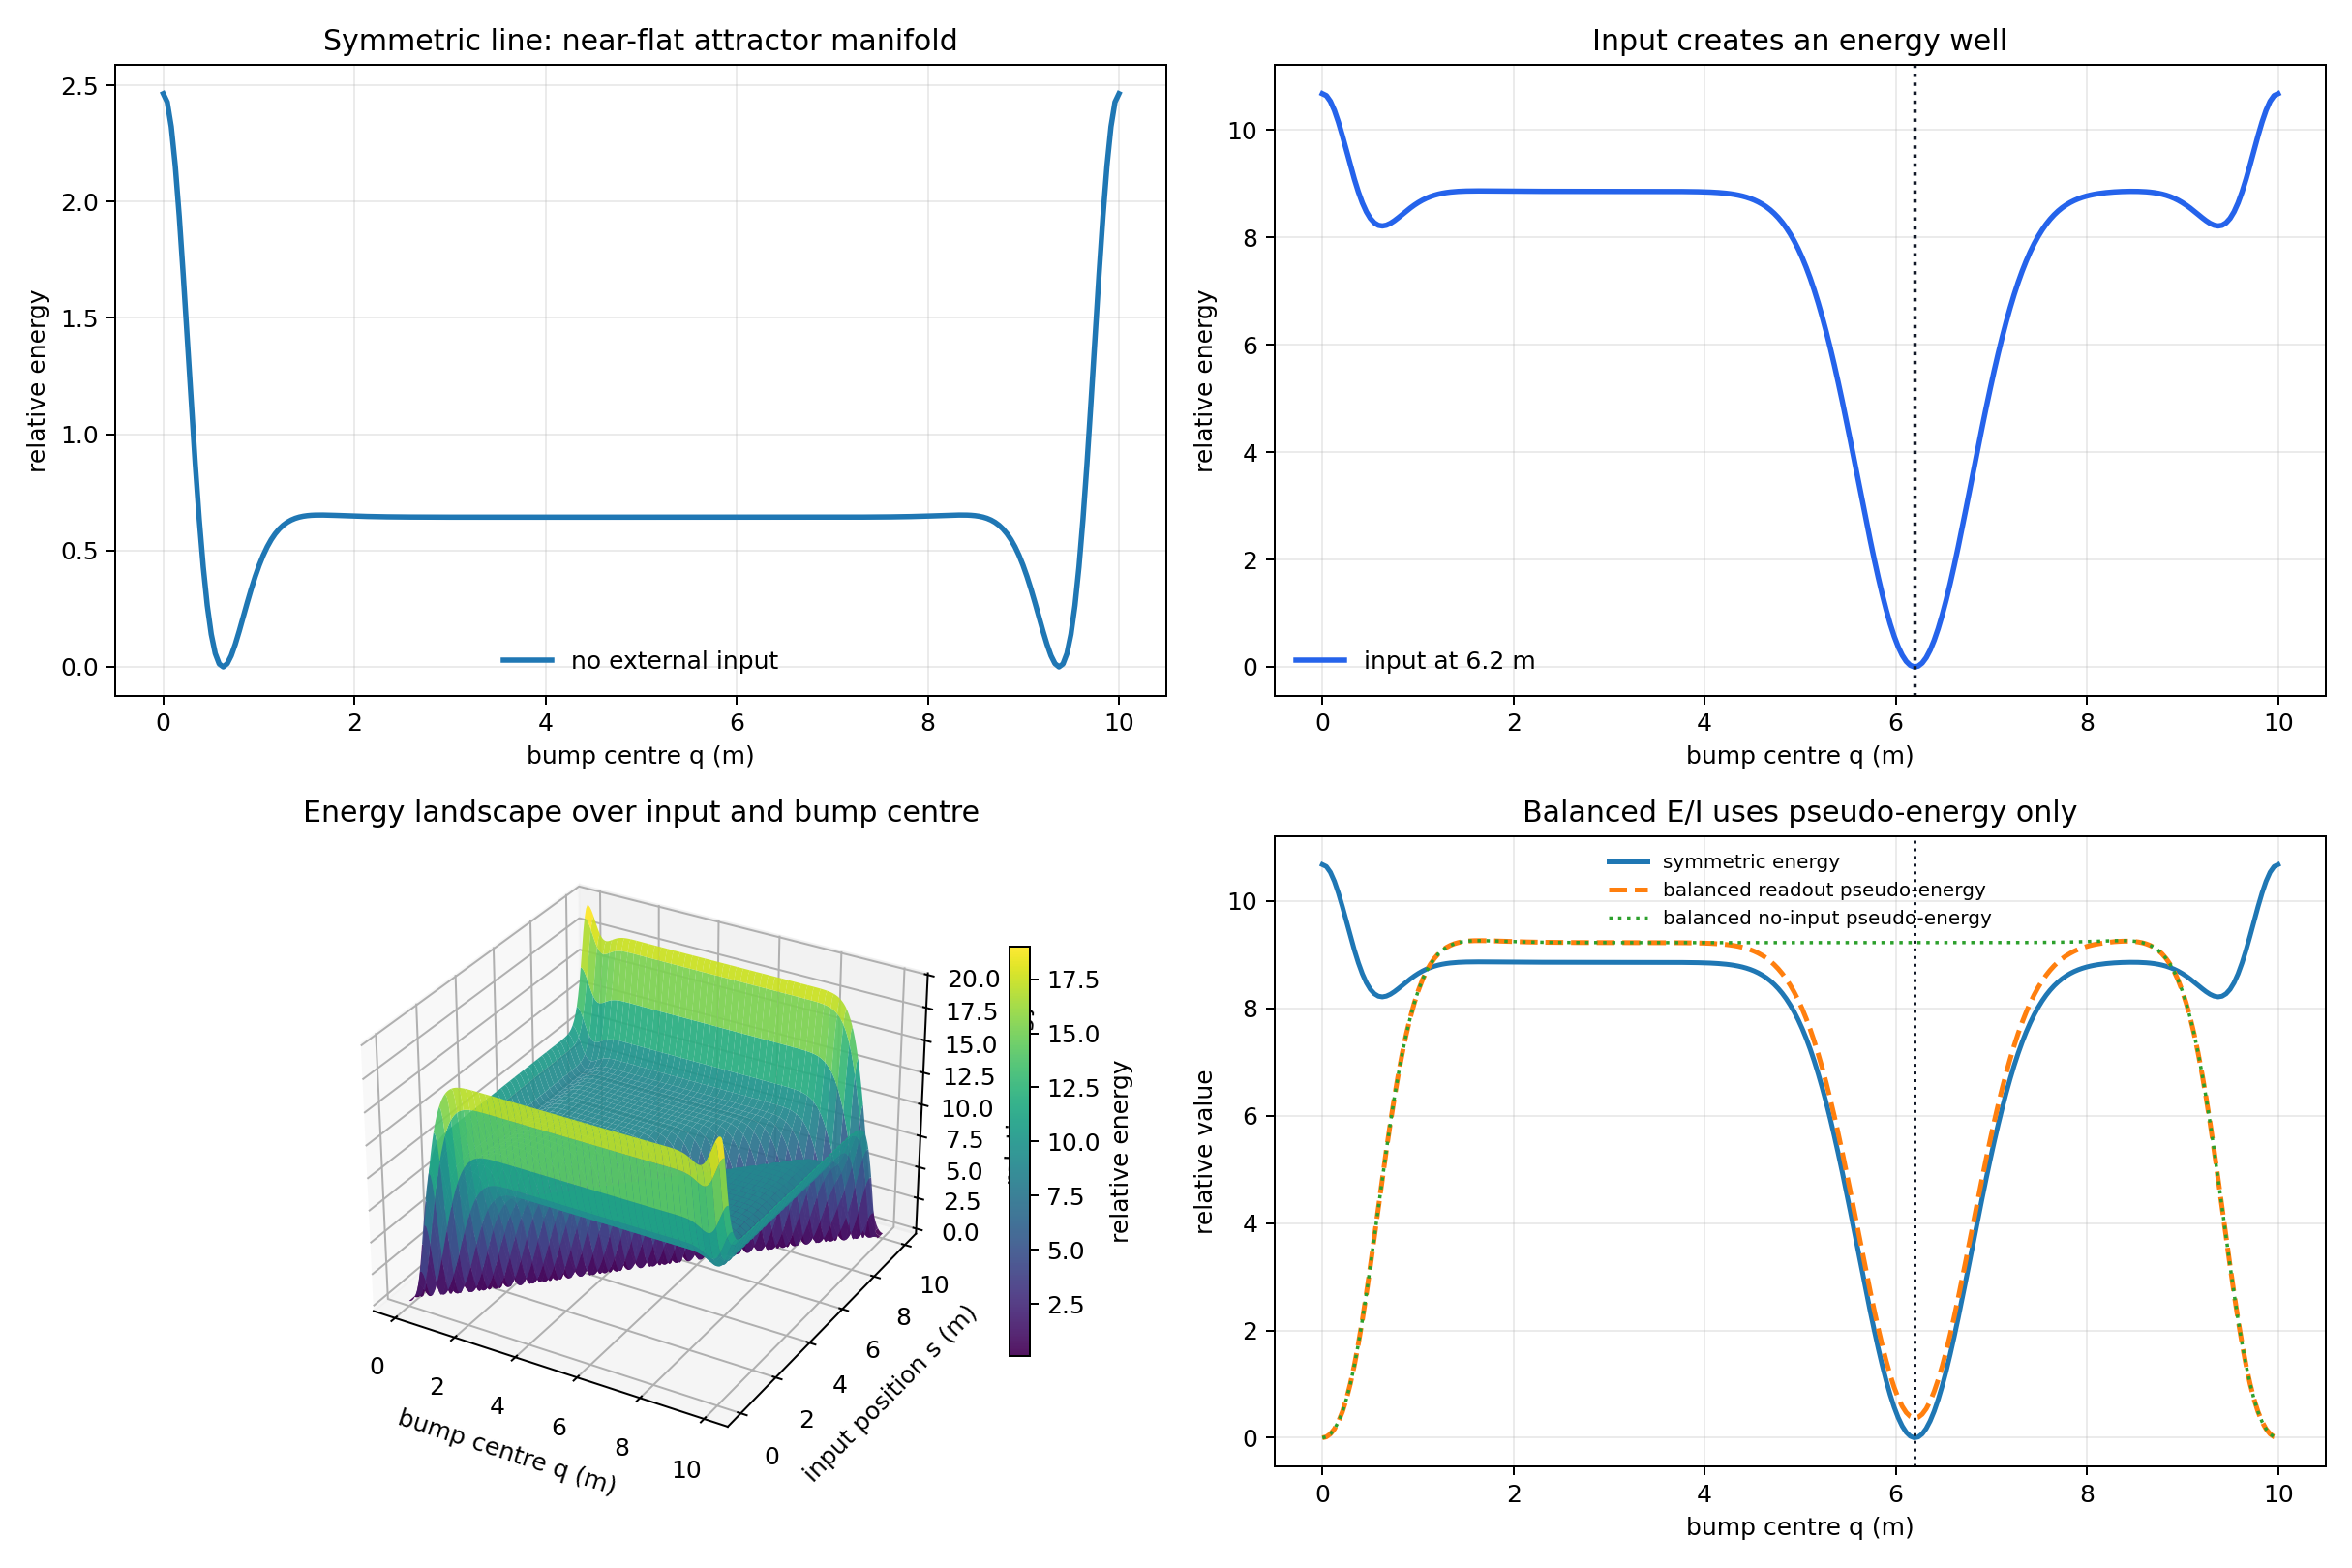
\includegraphics[width=\figwidth\linewidth]{ch5_energy_landscape.png}
  \caption{Illustrative energy landscape for the finite line attractor. The attractor should stabilise the bump without forcing all inputs to a single fixed point.}
\end{figure}

\section{Dynamics and Readout}

The attractor activity was decoded using a centre-of-mass or local population vector readout. For activity $r_i$ at represented coordinate $x_i$,
\[
  \hat{x}_{\mathrm{COM}} =
  \frac{\sum_i x_i r_i}{\sum_i r_i+\epsilon}.
\]
The local population vector restricts the sum to a neighbourhood around the peak. This can reduce distant tail effects, but it can also discard useful uncertainty information if the bump is broad.

\begin{figure}[H]
  \centering
  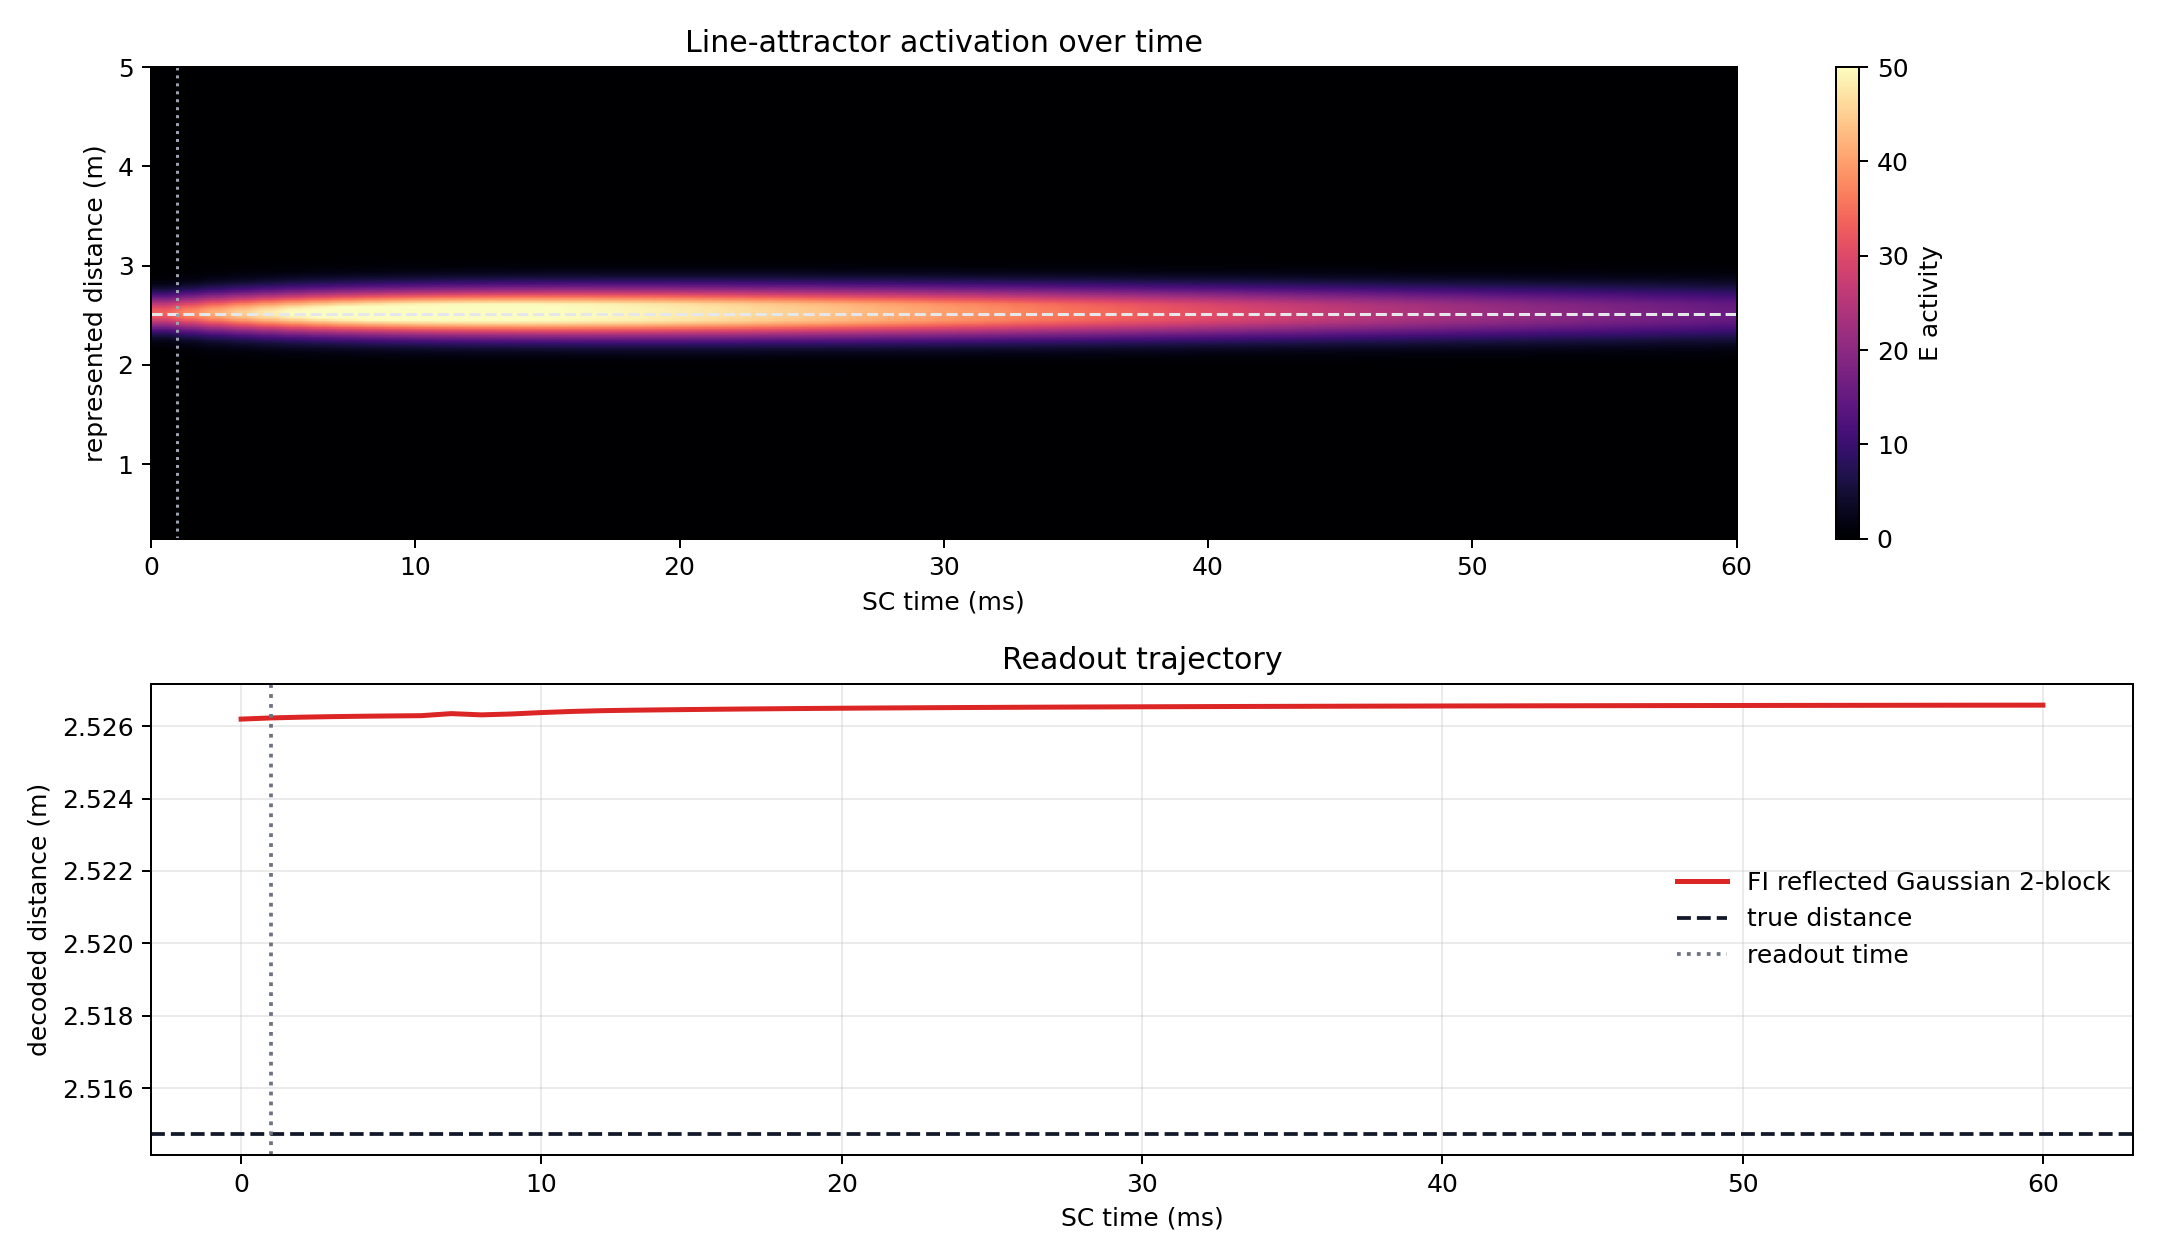
\includegraphics[width=\figwidth\linewidth]{ch5_line_attractor_dynamics.png}
  \caption{Line attractor bump dynamics. The activity forms a localised bump whose amplitude and width evolve over time.}
\end{figure}

\begin{figure}[H]
  \centering
  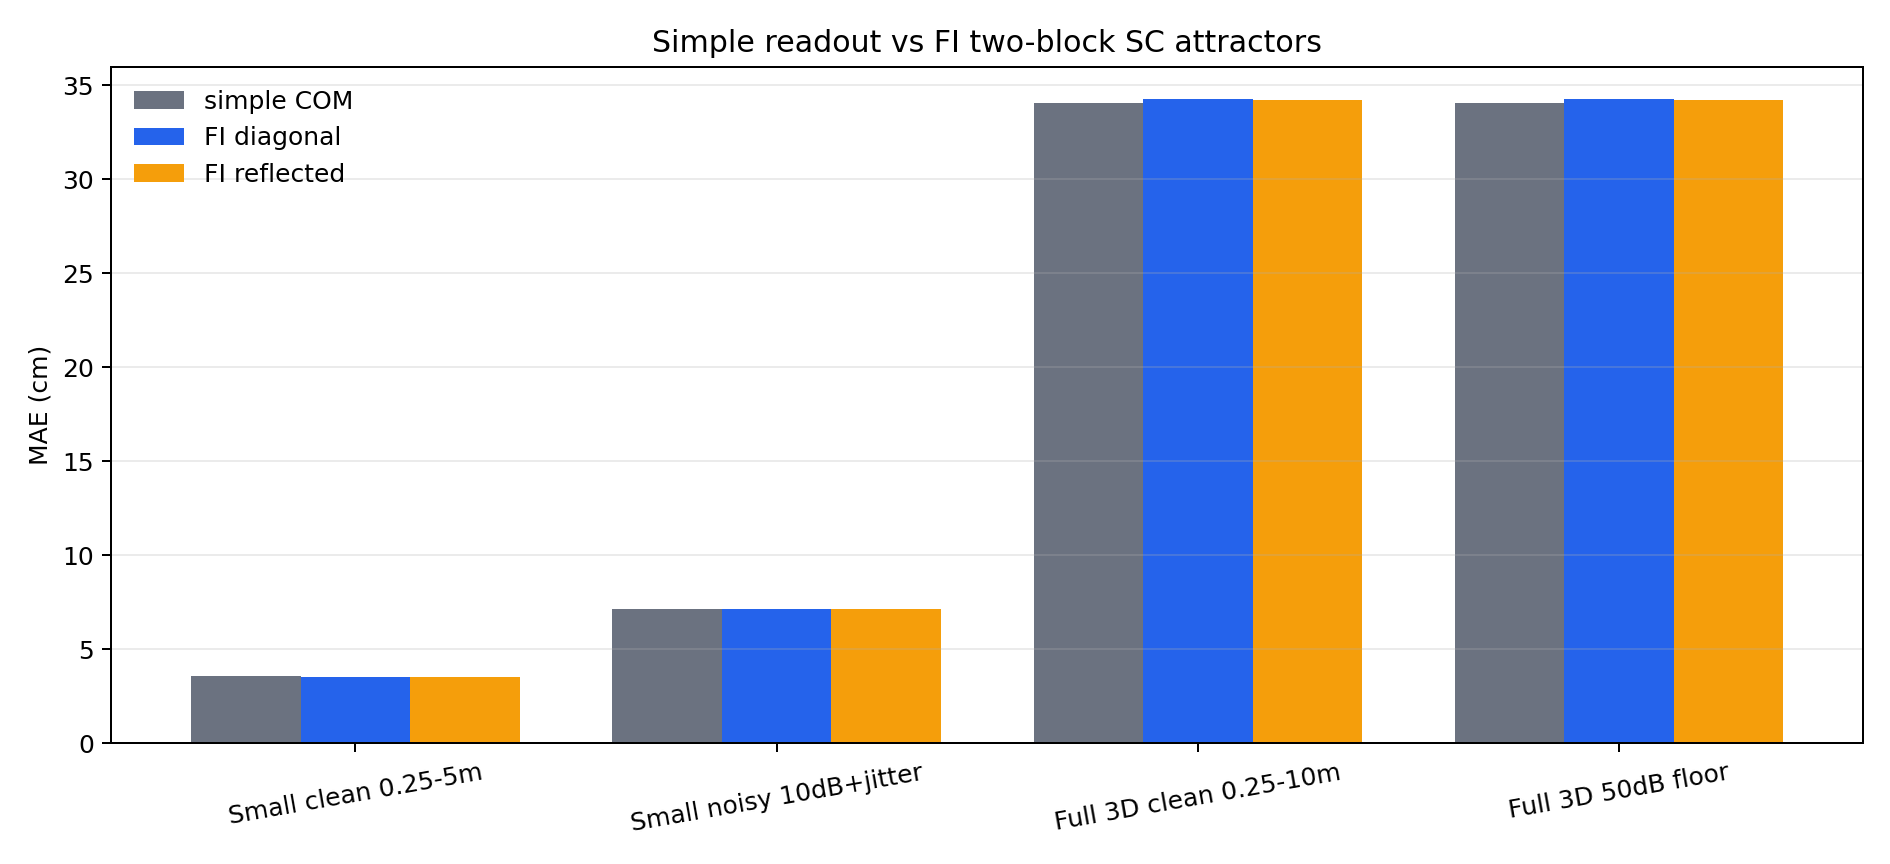
\includegraphics[width=\figwidth\linewidth]{ch5_readout_mae_comparison.png}
  \caption{Readout comparison for attractor and non-attractor variants. The attractor gives a structured stabilising readout, but the mean accuracy gains are modest in already clean cases.}
\end{figure}

\section{Biophysical Limits}

In an unconstrained mathematical model, increasing the recurrent gain parameter $\alpha$ can improve accuracy indefinitely by sharpening the bump. This is not biologically free. Higher gain implies higher firing rates, higher energy consumption, and greater risk of saturation. When rate caps are introduced, the gain advantage can disappear because the population cannot express the higher-amplitude bump. This motivates choosing moderate recurrent gain rather than simply maximising accuracy in an uncapped simulation.

\chapter{System-Level Performance and Discussion}

\section{Comparison with Earlier Models}

Earlier full trained models provide reference points. The best previous full trained variant was Round 3 Combined A, variant 2B+3, with combined error 0.0394, distance MAE 0.0646 m, azimuth MAE $2.86^\circ$, elevation MAE $2.53^\circ$, and Euclidean error 0.204 m. The Round 5 fixed ridge decoder achieved combined error 0.0387 and distance MAE 0.0438 m. These models are strong baselines because they exploit fixed features with trained or calibrated readouts.

\begin{table}[H]
  \centering
  \caption{Reference comparison with old combined models. Metrics are copied from the old experiment summaries.}
  \begin{tabular}{lllll}
    \toprule
    Model & Combined & Distance MAE & Azimuth MAE & Elevation MAE\\
    \midrule
    Round 3 2B+3 & 0.0394 & 0.0646 m & $2.86^\circ$ & $2.53^\circ$\\
    Round 4 combined & 0.0435 & 0.0786 m & $2.83^\circ$ & $2.78^\circ$\\
    Round 5 fixed ridge & 0.0387 & 0.0438 m & $3.11^\circ$ & $2.59^\circ$\\
    New distance pathway, full 3D up to 5 m & -- & 0.0266 m & -- & --\\
    New azimuth ILD, isolated $\pm45^\circ$ & -- & -- & $0.98^\circ$ & --\\
    New elevation DCN, full 3D up to 5 m & -- & -- & -- & $3.03^\circ$\\
    \bottomrule
  \end{tabular}
\end{table}

\section{Full-System Interpretation}

The new pathway results should not be overinterpreted as a completed end-to-end 3D system. The pathways have been developed and validated mostly independently. This is deliberate: the aim of the current stage is to establish biologically grounded, interpretable cue extractors before final integration. The distance pathway is now strong in the near field, the elevation pathway is competitive with old trained models, and the azimuth pathway is excellent in isolated conditions but breaks down under full three-dimensional confounds.

\begin{figure}[H]
  \centering
  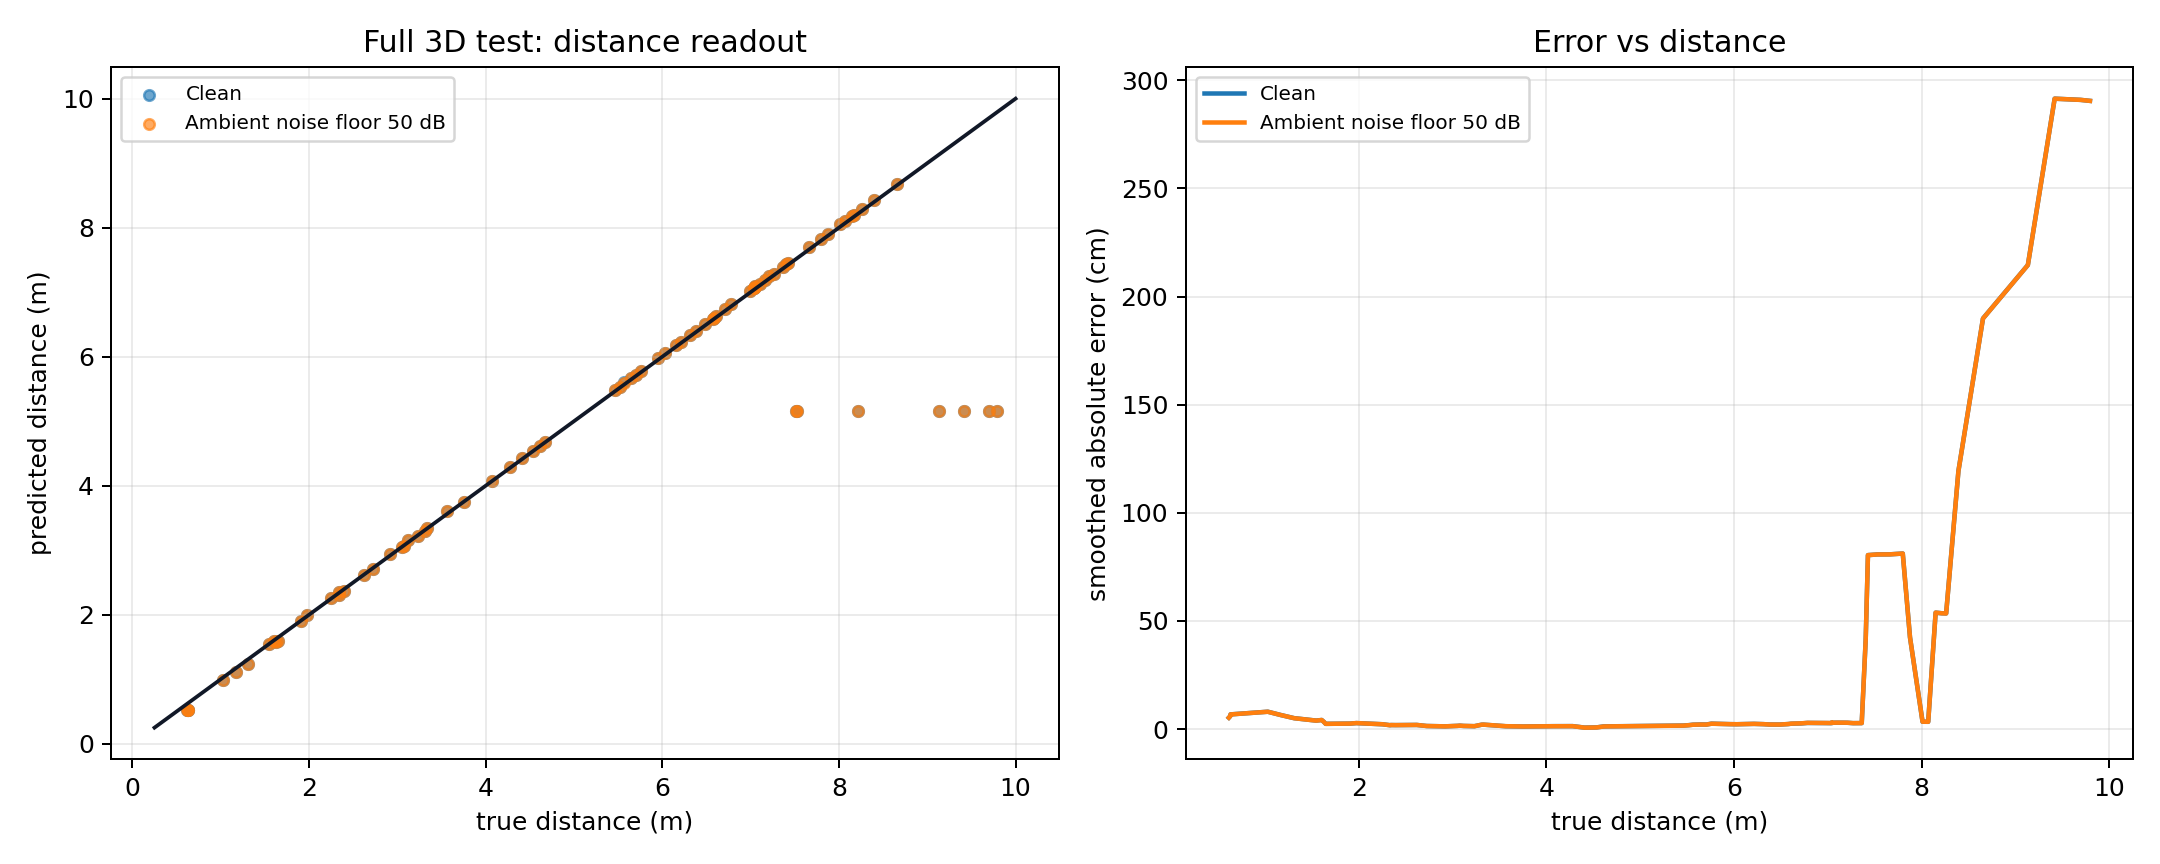
\includegraphics[width=\figwidth\linewidth]{ch6_distance_full_test_accuracy.png}
  \caption{Distance full-test accuracy. Performance remains strong up to 5 m, while the 10 m case exposes the limitations of the present near-field tuning.}
\end{figure}

\begin{figure}[H]
  \centering
  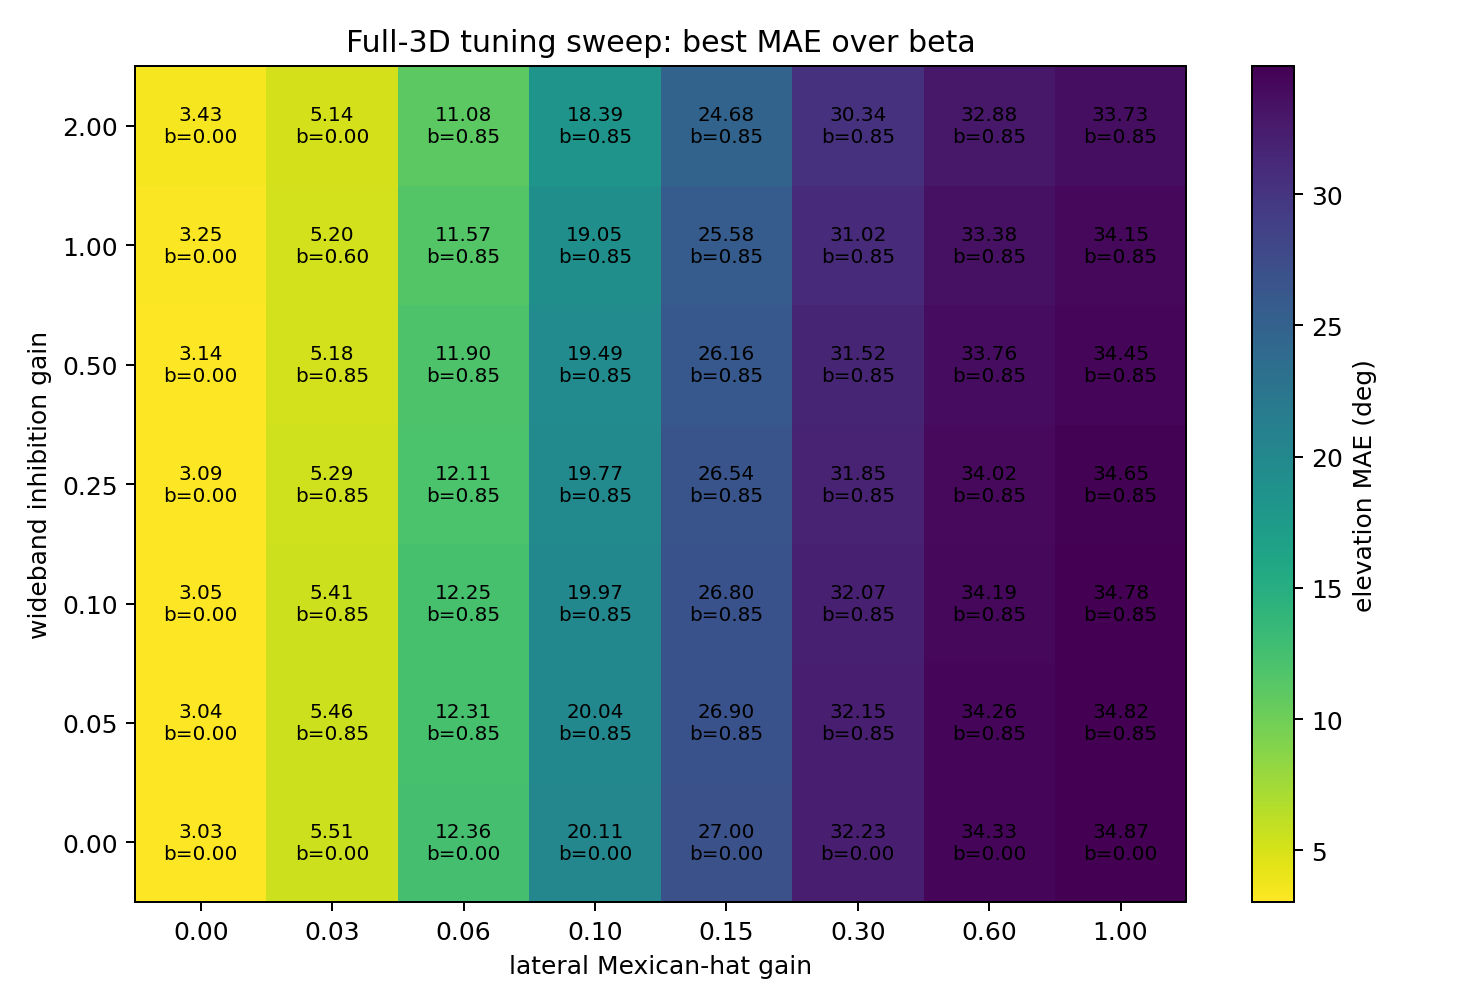
\includegraphics[width=\figwidth\linewidth]{ch6_elevation_tuning_sweep.png}
  \caption{Elevation tuning sweep. The best clean full-three-dimensional model was the deep-comb, signal-weighted DCN template without additional lateral or dynamic inhibition.}
\end{figure}

\section{Robustness}

Noise robustness was a major design constraint. The initial noisy distance tests failed because white noise created dense cochlear spikes, especially in sensitive low-frequency channels. The final fix combined cochlear threshold tuning, dynamic beta, channel silencing below 4 kHz, VCN consensus, and recalibrated latency. This sequence is a useful example of the bottom-up method: rather than adding a trained denoiser, the failure was traced to the biological stage where it arose.

Azimuth robustness remains less complete. The ILD branch is sensitive to any factor that changes the left/right amplitude ratio other than azimuth. Elevation spectral filtering, range-dependent attenuation, and noise can all distort the apparent ILD. The future integrated system should therefore combine ITD and ILD adaptively, and should condition the azimuth estimate on distance and elevation confidence.

\section{Environmental, Social, and Ethical Considerations}

The environmental motivation for this work is low-power sensing. Sparse event-based processing can reduce unnecessary computation and therefore energy use, particularly for always-on localisation systems. However, acoustic sensing also raises social and ethical issues. Active sonar emits sound into the environment, so operating frequency, intensity, and duty cycle must be chosen to avoid disturbance to humans and animals. If used in robotics or surveillance, the localisation system could also contribute to tracking people or objects without consent. A responsible deployment would need explicit limits on acoustic output power, data retention, and use context.

\section{Limitations}

The largest limitation is that the current system is not yet a fully integrated multi-object localiser. The distance, azimuth, and elevation pathways have been tested in increasingly realistic conditions, but final fusion and failure-case handling remain future work. The simulator is also simplified: head shadowing, comb filtering, attenuation, and noise are engineered approximations rather than measured bat HRTFs or room acoustics. Finally, the current performance is strongly tuned to the selected call, frequency band, and near-field range.

\chapter{Conclusions and Future Work}

\section{Conclusions}

This project shows that a modular neuromorphic echolocation system can be built from interpretable biological primitives. The final cochlea model provides sparse frequency-channel spikes at lower cost than the original FFT/IFFT approach. The distance pathway gives strong near-field range estimates using onset detection, corollary discharge, delay coincidence, and population readout. The azimuth pathway demonstrates that a simple ILD mechanism can be highly accurate after inverse-sigmoid warping, although it is confounded in full three-dimensional scenes. The elevation pathway demonstrates that a DCN-style synaptic template can decode comb-filter spectral notches with accuracy close to the old trained model.

The broader conclusion is methodological. Biological inspiration is most useful when it defines modular computations: filtering, onset sharpening, coincidence, inhibition, template matching, and attractor readout. These modules can be analysed, timed, stress-tested, and improved independently.

\section{Future Work}

The immediate next step is full pathway integration. The azimuth estimate should gate which ear contributes to elevation, while the distance estimate should help normalise amplitude-dependent cues. A second priority is failure-case analysis: the current reports identify several failure modes, but these should be formalised into a diagnostic suite. A third priority is targeted learning. Rather than training the whole system end-to-end, small calibration layers could be learned for the ILD warp, DCN template weighting, and final multi-cue fusion.

Longer-term extensions include multi-object tracking, velocity estimation, event-based hardware implementation, and measured HRTF replacement for the engineered head-shadow and comb-filter models.

\appendix

\chapter{Risk Assessment Retrospective}

This project was primarily computational and therefore carried low direct physical risk. The main practical risks were workstation strain, data loss, and mismanagement of long-running experiments. These were more significant than any laboratory hazard. In retrospect, the original risk assessment should have placed more explicit emphasis on software reproducibility, backup strategy, and compute-time management.

The project also raised indirect risks not usually captured by a safety form. Active acoustic localisation can disturb animals or humans if implemented physically at inappropriate sound pressure levels. The work here is simulation-based, but any future hardware version would need an acoustic exposure assessment. There are also ethical risks around localisation and tracking. If starting again, I would separate the risk assessment into three parts: immediate personal safety, computational project risk, and downstream deployment risk.

\chapter{Selected Pseudocode}

\section{Dynamic Cochlear Spike Encoding}

\begin{lstlisting}[language=Python,caption={Dynamic threshold and beta cochlear spiking.}]
for t in range(num_samples):
    threshold_t = threshold_inf + (threshold_0 - threshold_inf) * exp(-t / tau_threshold)
    beta_t = beta_inf - (beta_inf - beta_0) * exp(-t / tau_beta)
    v = beta_t * v + channel_envelope[:, t]
    spikes[:, t] = v >= threshold_t
    v = v - spikes[:, t] * threshold_t
spikes[centre_frequencies < 4000, :] = 0
\end{lstlisting}

\section{Distance Coincidence Detector}

\begin{lstlisting}[language=Python,caption={Delay-line coincidence scoring.}]
for k, delay in enumerate(candidate_delays):
    shifted_cd = shift(corollary_discharge, delay)
    score[k] = sum(vcn_spikes & shifted_cd)
ac_activity = mexican_hat_filter(score)
distance_hat = sum(distance_grid * ac_activity) / sum(ac_activity)
\end{lstlisting}

\section{Elevation Template Matching}

\begin{lstlisting}[language=Python,caption={Signal-weighted DCN elevation template.}]
for theta in elevation_grid:
    H_theta = comb_transfer_function(frequencies, lag(theta), gain)
    template[theta] = baseline_signal_power * abs(H_theta) ** 2
    template[theta] = normalise(template[theta])

dcn_activity = template @ cochlear_power
elevation_hat = centre_of_mass(elevation_grid, dcn_activity)
\end{lstlisting}

\chapter{Notes for Final Editing}

This draft should be compressed before submission. The final report limit is 53 A4 pages total, including title page and technical abstract. The most likely compression strategy is:
\begin{itemize}
  \item move detailed derivations into appendices;
  \item keep only the strongest pathway figures in the main text;
  \item combine pathway result tables;
  \item remove implementation details that are already clear from equations and pseudocode;
  \item use the technical abstract for results summary, not for detailed motivation.
\end{itemize}

\begin{thebibliography}{9}
\bibitem{gerstner}
W. Gerstner, W. Kistler, R. Naud, and L. Paninski, \textit{Neuronal Dynamics}. Cambridge University Press, 2014.

\bibitem{dayanabbott}
P. Dayan and L. Abbott, \textit{Theoretical Neuroscience}. MIT Press, 2001.

\bibitem{jeffress}
L. A. Jeffress, ``A place theory of sound localization,'' \textit{Journal of Comparative and Physiological Psychology}, 1948.

\bibitem{cann}
S. Amari, ``Dynamics of pattern formation in lateral-inhibition type neural fields,'' \textit{Biological Cybernetics}, 1977.

\bibitem{bat}
J. A. Simmons and R. A. Stein, ``Acoustic imaging in bat sonar,'' \textit{Journal of Comparative Physiology}, 1980.
\end{thebibliography}

\end{document}
